\documentclass[runningheads]{llncs}

% Required packages from ECML-PKDD template
\usepackage[T1]{fontenc}
\usepackage{graphicx}
\usepackage{booktabs}
\usepackage[misc]{ifsym}
\newcommand{\corr}{(\Letter)}

% Additional packages (compatible with llncs)
\usepackage{amsmath}
\usepackage{amssymb}
\usepackage{multirow}
\usepackage{enumitem}
\usepackage{float}
\usepackage{adjustbox}
\usepackage{hyperref}
\usepackage{xcolor}
\usepackage{url}
\usepackage{longtable}
% \usepackage{microtype}  % Removed - incompatible with llncs

% Line spacing - llncs compliant
\setlength{\textfloatsep}{6pt plus 2pt minus 2pt}
\setlength{\dbltextfloatsep}{6pt plus 2pt minus 2pt}

\begin{document}

\title{FIG-MAC: A Fine-grained Inspiration Graph Empowered Multi-Agent Collaboration for Automated Scientific Hypothesis Generation}

\titlerunning{FIG-MAC for ASHG}

\author{First Author \and Second Author \and Third Author}

\authorrunning{F. Author et al.}

\institute{Affiliation/Address line 1 \\
Affiliation/Address line 2 \\
\email{email@domain}}

\maketitle

\begin{abstract}
Automated Scientific Hypothesis Generation (ASHG) leveraging large language models (LLMs) aims to harness their strengths in knowledge integration, logical reasoning, and text generation for efficiently producing innovative, verifiable scientific hypotheses. However, existing approaches face three critical limitations: (i) insufficient fine-grained knowledge construction, where noise in unstructured documents impairs LLM comprehension and reasoning; (ii) lack of knowledge evolution traceability, as current retrieval relies on superficial semantic or citation links without modeling knowledge origins and trajectories; (iii) absence of human-inspired and role-specialized multi-agent collaboration, to complete the full ASHG-evaluation loop. To address these limitations, we propose the Fine-grained Inspiration Graph-empowered Multi-Agent Collaboration framework (FIG-MAC) including: (i) Fine-grained Inspiration Graph module (FIG), to obtain fine-grained structured knowledge representations, where nodes represent academic semantic units and edges encode heuristic relationships among them; (ii) "Skeleton-Flesh" hybrid reasoning module, fusing FIG-based graph path reasoning as a structural backbone with vector search as semantic enrichment, enabling the discovery of traceable scientific conjecture paths; (iii) role-specialized multi-agent framework, inspired by real scientific teamwork, enabling a closed-loop process of scientific conjecture generation, screening, and validation. Experiments on 150 research questions demonstrate that FIG-MAC achieves the highest source diversity ($U_{\text{src}}=0.650$), provenance-adjusted novelty ($P=0.535$), and raw novelty (ON$_{\text{raw}}=0.684$), significantly outperforming baselines in cross-domain knowledge integration across AI subfields (e.g., computer vision, NLP, graph learning). Our code is available at \href{https://github.com/SiyuanChenToDo/KG-LLM.git}{GitHub repository}.

\keywords{Scientific Hypothesis Generation, Multi-Agent Collaboration, Knowledge Graphs, Large Language Models}
\end{abstract}

\section{Introduction}

Automated Scientific Hypothesis Generation (ASHG) based on large language models (LLMs) aims to leverage their robust capabilities in knowledge integration, logical reasoning, and text generation to efficiently produce innovative and verifiable scientific hypotheses~\cite{DBLP:journals/tmlr/AgarwalSPLDSCP25,DBLP:journals/pr/LiuZWL26}. As illustrated in Figure~\ref{fig1}, such methods have achieved initial success in multiple domains, including the prediction of chemical molecular properties~\cite{yang2024moose,yang2025moose2}, the formulation of physical theoretical conjectures, the screening of novel semiconductor materials, and the mining of potential drug molecules.

\begin{figure}[t]
    \centering 
    
\includegraphics[width=1\textwidth]{fig1.pdf} 
    \caption{The Wide-Ranging Applications of ASHG Across Diverse Domains.}
    \label{fig1}
\end{figure}

In recent years, ASHG has focused on three domains: (1) to identify potential research gaps in academic literature, models such as AutoResearcher~\cite{DBLP:journals/corr/abs-2510-20844}, HypoGen~\cite{zhou2024hypothesis}, and MC-NEST~\cite{DBLP:journals/corr/abs-2411-15645} have detected research blind spots by integrating knowledge retrieval and logical reasoning; (2) to improve the empirical feasibility and verifiability of generated hypotheses, recent methods explicitly optimize hypotheses for testability and practical relevance, AI Scientist systems~\cite{DBLP:journals/corr/abs-2408-06292,aiscientist_v2} operationalize hypothesis generation as an iterative ``proposing-evaluating-refining'' loop, Causal Graph-guided approaches~\cite{tong2024automating} constrain hypothesis space using explicit causal structures, while LLM-based iterative optimization~\cite{rabby2025iterative} progressively refines hypotheses via feedback-driven reasoning and evaluation; (3) to improve the factual consistency and verifiability of hypotheses, techniques including Retrieval-Augmented Generation (RAG)~\cite{DBLP:conf/nips/LewisPPPKGKLYR020} and Graph Reasoning~\cite{liang2024survey} have been integrated to enhance the scientific rigor and reliability of hypotheses.

However, the following limitations remain: (1) lack of fine-grained academic knowledge representation: Most existing external knowledge exists in the form of unstructured documents or abstracts, which contain substantial noise and thus affect the subsequent comprehension and reasoning accuracy of LLMs; (2) insufficient traceability of knowledge evolution: Current knowledge retrieval relies on surface-level semantic similarity or citation associations, lacking modeling of the origin and development path of knowledge. This makes it difficult for models to understand the dynamic process of ASHG and restricts their ability to break through the boundaries of existing problems; (3) absence of structured, role-aware multi-agent collaboration: Single agent cannot independently complete the full-process closed loop from problem discovery and reasoning generation to hypothesis evaluation. Insufficient exploration of multi-agent collaboration mechanisms has hindered the large-scale practical deployment of ASHG methods.

To address these challenges, we propose the Fine-grained Inspiration Graph-empowered Multi-Agent Collaboration framework (FIG-MAC). First, the \textbf{Fine-grained Inspiration Graph module (FIG)} converts raw corpus into semantic units through knowledge parsing and constructs heuristic relationships between these units, providing structured knowledge for reasoning. Second, the \textbf{`Skeleton-Flesh' hybrid reasoning module} generates knowledge skeleton evolution paths via graph traversal, and supplements specific content (the ``flesh'') for each node by combining vector retrieval, forming a traceable dynamic knowledge context. Finally, the \textbf{role-specialized multi-agent framework} simulates the real scientific research process by setting intelligent roles such as knowledge exploration, idea generation, and parallel domain review. Through multiple rounds of evaluation and knowledge interpretability feedback, the framework generates rigorously verified scientific hypotheses.

Extensive experiments demonstrate that FIG-MAC achieves competitive performance across multiple dimensions: highest source diversity ($U_{\text{src}}=0.650$ vs. 0.512 for COI Agent), provenance-adjusted novelty ($P=0.535$ vs. 0.345 for COI Agent), and raw overall novelty (ON$_{\text{raw}}=0.684$), while maintaining strong source quality ($S_{\text{src}}=0.276$). These results validate the effectiveness of graph-enhanced hybrid reasoning for generating hypotheses that are both structurally novel and technically grounded. Our contributions are summarized as follows:

\noindent\textbullet\ We construct a specialized multi-agent collaboration framework that achieves a full-process, interpretable closed loop for ASHG and verification.

\noindent\textbullet\ We propose a fine-grained inspiration graph module that enables structured denoising and semantic enhancement of knowledge with Inspired edges capturing cross-paper innovation mechanisms.

\noindent\textbullet\ We design a ``skeleton-flesh'' reasoning mechanism that enhances the dynamic traceability of ASHG.


\section{Related Work}

\subsection{Scientific Hypothesis Generation}
Automated scientific hypothesis generation has evolved across methodological paradigms. Literature-Based Discovery (LBD), is rooted in "undiscovered public knowledge" and the ABC model, which infers relationships between concepts $A$ and $C$ via shared intermediate concepts $B$ \cite{swanson1986fish,swanson1986undiscovered}. Recent LLM-based approaches enhance hypothesis generation through agentic frameworks \cite{wang2024research,si2024large,baek2025research}, but neglect retrieval quality, limiting hypothesis novelty, validity and diversity \cite{lewis2020retrieval,zhao2024survey,li2024b}. While some methods incorporate knowledge subgraphs, citation neighbors or semantically similar works \cite{wang2024research,li2024b,baek2025research}, seed paper abstracts (containing methodology/results) introduce retrieval bias and reduce idea novelty.

\subsection{Retrieval for Scientific Discovery}
Scientific paper retrieval employs queries like abstracts/titles \cite{singh2023scincl,ostendorff2022neighborhood,cohan2020specter}, keywords \cite{sesagiri2017full}, textual queries \cite{anand2017proposed,parisot2022scientific,medic2023similarity} or paper aspects \cite{singh2024scispace,singh2023scincl,mysore2022multi,ostendorff2022s2orc}, relying on semantic similarity for representation learning. However, mainstream retrieval models (sentence-based similarity \cite{reimers2019sentence,beltagy2019scibert} or generic inter-document embedding \cite{cohan2020specter,singh2022specter2}) often yield irrelevant results (e.g., keyword overlap). Recent studies highlight semantic similarity's ineffectiveness for scientific retrieval \cite{yang2024c}, emphasizing the need for deeper analysis of solution applicability to target problems.

\subsection{Reasoning-Intensive Retrieval}
Traditional information retrieval focuses on keyword matching \cite{robertson2009probabilistic} or semantic matching \cite{devlin2019bert}, ignoring reasoning-intensive queries. Benchmarks like BRIGHT \cite{su2024bright} and RAR-b \cite{xiao2024rar} reveal this gap. Chain-of-thought retrieval \cite{trivedi2023interleaving} faces challenges in constructing effective reasoning sequences; LLM-based re-rankers \cite{niu2024rankgpt,yang2024c} and instruction-following methods \cite{weller2024follow,weller2024prompting} are either impractical (high cost for large corpora) or ineffective (retrievers perform poorly with reasoning instructions \cite{xiao2024rar}). Contrastive training is explored to adapt retrievers for reasoning tasks \cite{shao2025reasonir}.

\subsection{Knowledge Graph and Multi-Agent Methods}
Knowledge graph-based approaches frame hypothesis generation as link prediction over structured scientific knowledge \cite{borrego2025research,de2021discovering}. Early academic knowledge graphs (Semantic Scholar \cite{ammar2018construction}, Microsoft Academic Graph \cite{wang2020microsoft}) model coarse-grained entities (papers, authors, venues) and citations, while recent work focuses on fine-grained entity/relationship modeling \cite{luan2018multi} for precise hypothesis generation. Graph embedding methods score hypothesis plausibility via low-dimensional entity/relation representations \cite{rossi2021knowledge,wang2021survey}.

Multi-agent systems enable collaborative hypothesis generation/validation by distributing roles (generation, critique, refinement) across specialized agents \cite{ghafarollahi2025sciagents,ke2025biodisco}. SciAgents integrates ontological knowledge graphs with LLMs via specialized agents (Ontologist, Scientists, Critic) \cite{ghafarollahi2025sciagents}, and frameworks like POPPER implement agentic validation based on falsification \cite{huang2025automated}.

\subsection{Limitations of Current Approaches}
Existing methods suffer from critical limitations: over-reliance on shallow semantic similarity/static graph links (ignoring dynamic knowledge evolution and closed-loop evaluation), lack of unified frameworks for discovery, reasoning traceability and multi-agent evaluation, and separation of hypothesis generation/validation (hindering iterative refinement via empirical feedback). Our work addresses these gaps with an integrated framework combining fine-grained knowledge construction, traceable reasoning paths, and role-specialized multi-agent collaboration for hypothesis generation and validation.


\section{Methodology}
\label{sec:methodology}

We propose FIG-MAC, a collaborative multi-agent framework designed for ASHG by simulating the reasoning process of human research teams. FIG-MAC comprises three components, as shown in Figure~\ref{fig2}: (i) the \textbf{Fine-grained Inspiration Graph module (FIG)} that provides structured knowledge representation; (ii) the \textbf{"Skeleton-Flesh" hybrid reasoning module} that combines semantic vector search with graph-based structural reasoning; and (iii) the \textbf{role-specialized multi-agent framework} that orchestrates specialized agents through iterative hypothesis refinement workflows.

\textbf{Notation.} Throughout this section, we use the following notation: $\mathcal{G} = (\mathcal{V}, \mathcal{E}, \mathcal{R})$ denotes a heterogeneous knowledge graph with node set $\mathcal{V}$, edge set $\mathcal{E}$, and relation type set $\mathcal{R}$; $\mathcal{C}$ denotes the shared context space containing retrieval evidence and inter-agent messages; bold uppercase letters (e.g., $\mathbf{W}$, $\mathbf{h}$) represent matrices and vectors; calligraphic letters (e.g., $\mathcal{S}$, $\mathcal{A}$) denote sets and spaces; subscripts indicate entity indices (e.g., $i$, $j$) or relation types (e.g., $r$); superscripts in parentheses (e.g., $^{(l)}$, $^{(t)}$) indicate layer numbers or time steps.

\begin{figure*}[t] 
\centering
    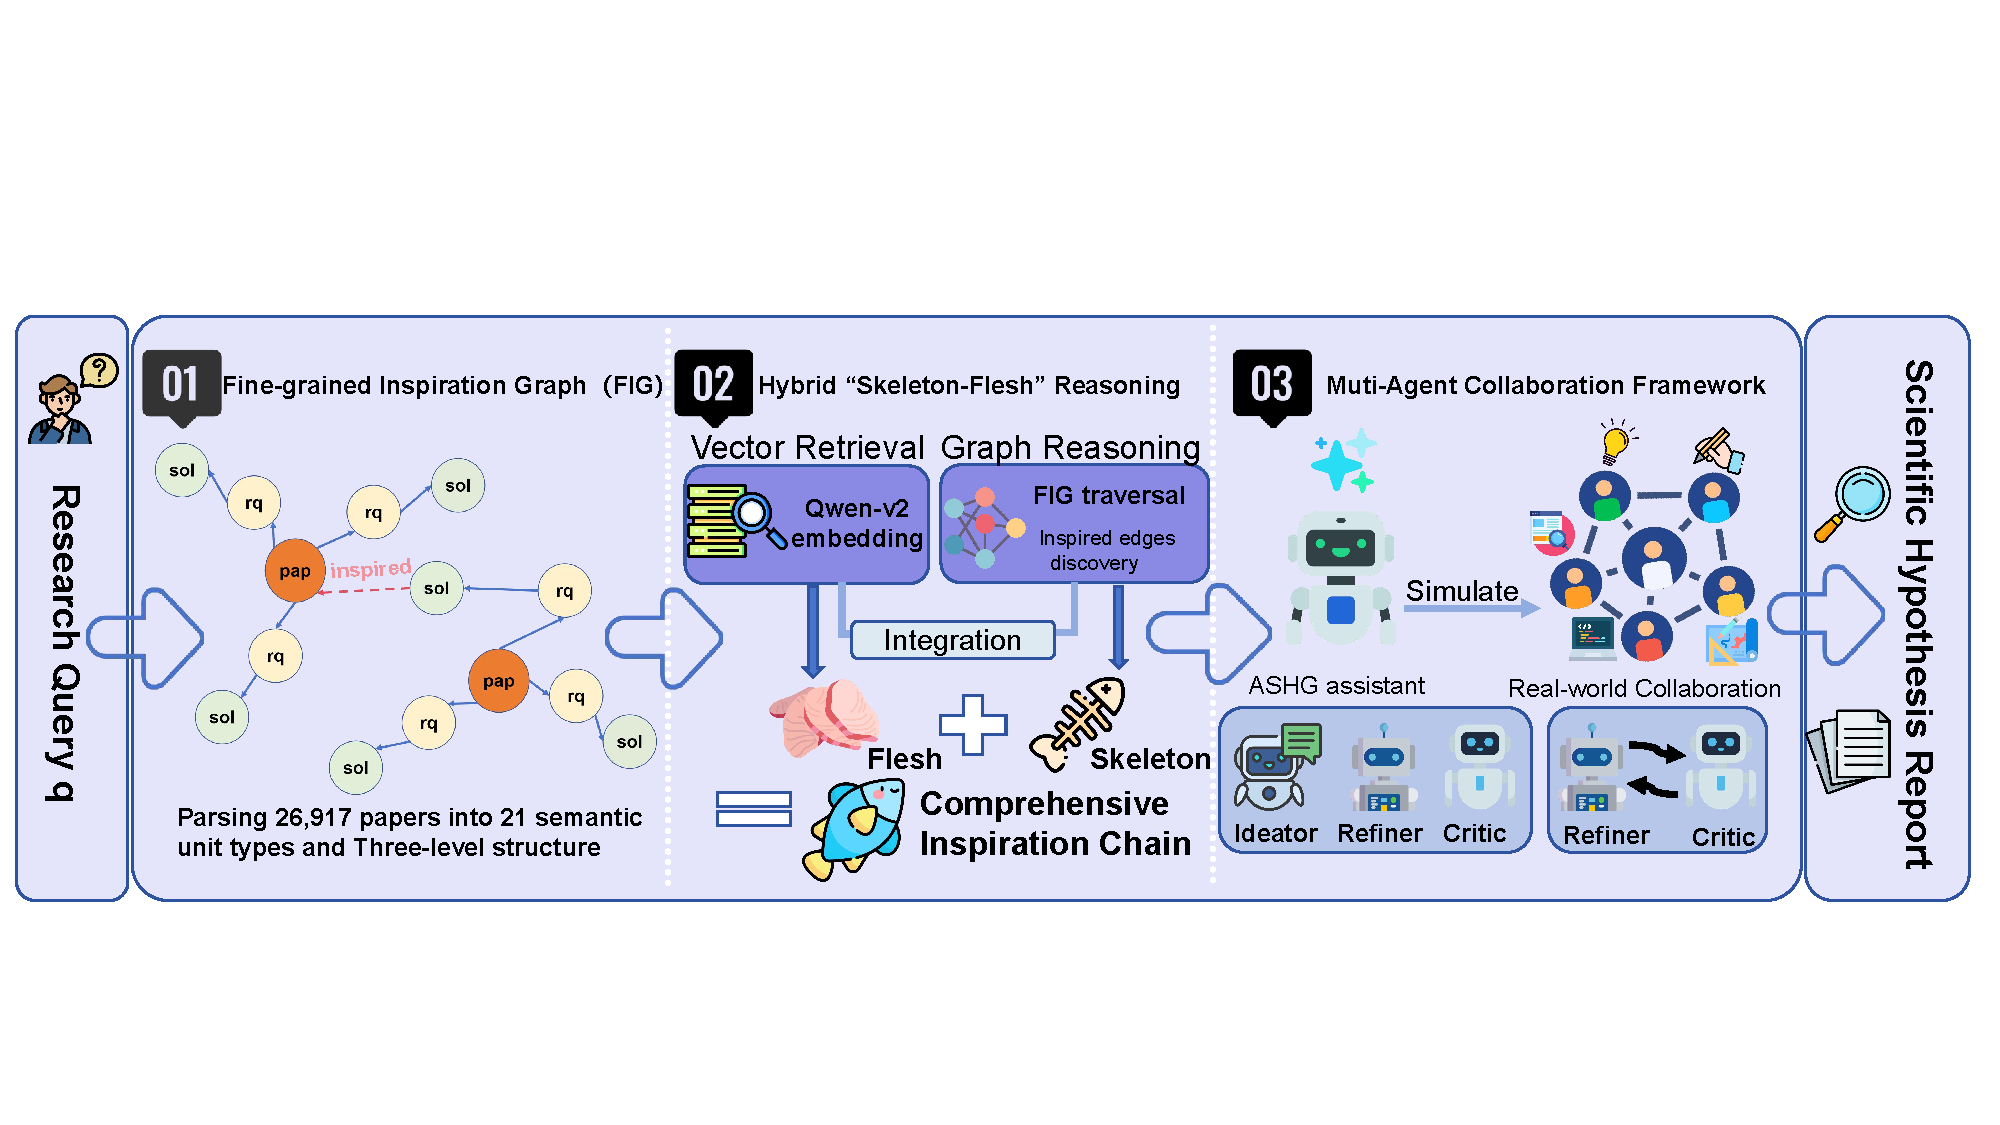
\includegraphics[width=1\textwidth]{fig2.pdf} 
    \caption{Fine-grained Inspiration Graph-based Multi-Agent Collaboration (FIG-MAC).}
    \label{fig2}
\end{figure*}

\subsection{Fine-grained Inspiration Graph Construction}
\label{sec:graph_construction}

To enable structured knowledge representation that captures fine-grained academic semantics and cross-paper innovation pathways, we design the Fine-grained Inspiration Graph (FIG). Unlike traditional paper-level citation networks, FIG decomposes scientific literature into semantic units and models their relationships at multiple granularities. Formally, FIG is a heterogeneous knowledge graph denoted as $\mathcal{G} = (\mathcal{V}, \mathcal{E}, \mathcal{R})$, where $\mathcal{V}$ represents the set of nodes, $\mathcal{E}$ denotes the set of edges, and $\mathcal{R}$ is the set of relation types. The current implementation encodes 26,917 papers from five conferences (2019--2024), yielding three primary entity types: Papers ($PAP$), Research Questions ($RQ$), and Solutions ($SOL$).

\textbf{Fine-grained Data Structuring.} The core challenge lies in accurately extracting key information and core entities from raw text. We perform fine-grained structured parsing on each paper, dividing the full text into 21 semantic units. This ultimately forms a three-level knowledge structure centered on the core entities "PAP - RQ - SOL", with the remaining semantic units serving as supplementary attributes.

\textbf{Entity Extraction.} We employ a two-stage pipeline to ensure parsing quality. First, 500 papers are manually annotated and refined to standardized samples, which fine-tune a Qwen-based extractor. This model then processes the full corpus, generating structured semantic units for each paper.

% \textbf{Relation Construction.} FIG encodes two relation classes: (1) Hierarchical relations $r_{\text{has\_rq}}$ and $r_{\text{has\_sol}}$ mapping intra-paper structures, where each paper contains approximately 3 research questions on average; and (2) Cross-paper relations $r_{\text{related}}$ and $r_{\text{inspired}}$ capturing inter-paper influences. To construct cross-paper edges at scale, we combine similarity filtering with supervised classification. Specifically, 1,550 entity pairs are manually labeled by three experts (Kappa$=0.85$) into three categories: Related, Inspired, or Irrelevant. Pairs with similarity below threshold $\eta = 0.5788$ (determined from the Irrelevant distribution) are pruned. Remaining candidates are classified by a fine-tuned Qwen3-8B (validation accuracy 95.52\%), yielding $|\mathcal{E}| = 1{,}809{,}779$ edges: 1,269,774 Related (70.16\%) and 540,005 Inspired (29.84\%). Critically, $r_{\text{inspired}}$ edges explicitly model how $SOL$ in one paper inspire $RQ$ or methodologies in another, capturing innovation pathways invisible to citation analysis.
\textbf{Relation Construction.} FIG encodes two relation classes: (1) Hierarchical relations $r_{\text{has\_rq}}$ and $r_{\text{has\_sol}}$ mapping intra-paper structures, where each paper contains approximately 3 research questions on average; and (2) Cross-paper relations $r_{\text{related}}$ and $r_{\text{inspired}}$ capturing inter-paper influences. To construct cross-paper edges at scale, we combine similarity filtering with supervised classification. Samples are manually labeled by three experts into three categories: Related, Inspired, or Irrelevant. Pairs with similarity below threshold are pruned. Remaining candidates are classified by a fine-tuned Qwen3-8B. Critically, $r_{\text{inspired}}$ edges explicitly model how $SOL$ in one paper inspire $RQ$ or methodologies in another, capturing innovation pathways invisible to citation analysis.

To discover non-obvious inspiration paths, we employ a Relation Graph Convolutional Network (RGCN) for representation learning. Let $\mathbf{h}_i^{(l)} \in \mathbb{R}^d$ denote the embedding of node $i$ at layer $l$, where $d$ is the embedding dimension. The RGCN update rule is:
\begin{equation}
    \mathbf{h}_i^{(l+1)} = \sigma \Bigg( \sum_{r \in \mathcal{R}} \sum_{j \in \mathcal{N}_r(i)} \frac{1}{c_{i,r}} \mathbf{W}_r^{(l)} \mathbf{h}_j^{(l)} + \mathbf{W}_0^{(l)} \mathbf{h}_i^{(l)} \Bigg),
\end{equation}
where $\mathcal{N}_r(i) = \{j \mid (j, i, r) \in \mathcal{E}\}$ denotes the set of neighbors of node $i$ under relation $r \in \mathcal{R}$; $\mathbf{W}_r^{(l)} \in \mathbb{R}^{d \times d}$ is the relation-specific weight matrix at layer $l$; $\mathbf{W}_0^{(l)} \in \mathbb{R}^{d \times d}$ is the self-connection weight matrix; $c_{i,r} = |\mathcal{N}_r(i)|$ is the normalization constant (node degree); and $\sigma(\cdot)$ is the activation function (ReLU).

After $L$ layers, we obtain final node embeddings $\mathbf{h}_i^L$. These are decoded via the DistMult scoring function to predict missing links:
\begin{equation}
    s(u, r, v) = (\mathbf{h}_u^L)^T \mathbf{R}_r \mathbf{h}_v^L,
\end{equation}
where $\mathbf{R}_r \in \mathbb{R}^{d \times d}$ is a learnable diagonal matrix representing relation $r$. High-scoring triplets are extracted via beam search to form inspiration chains $\pi = \{(v_1, r_1, v_2), (v_2, r_2, v_3), \ldots\}$, connecting source paper solutions to target research questions via intermediate nodes.

\subsection{"Skeleton-Flesh" Hybrid Reasoning Module}
\label{sec:hybrid_reasoning}

To achieve deep, traceable reasoning that combines the semantic richness of dense retrieval with the structural insights of graph traversal, we propose a Hybrid ``Skeleton-Flesh'' Reasoning method. This approach integrates two complementary retrieval paradigms: graph-based path discovery provides the ``skeleton'' of cross-domain knowledge evolution, while vector-based semantic search provides the ``flesh'' of domain-specific technical details. Given a research query $Q$, two retrieval functions operate in parallel: (1) Vector Retrieval $\mathcal{R}_V(Q)$ identifies topically relevant papers via dense embeddings, returning papers ranked by semantic similarity; (2) Graph Retrieval $\mathcal{R}_G(Q)$ traverses FIG to extract inspiration chains $\pi$ connecting $Q$ to $\text{SOL}$ nodes through $r_{\text{inspired}}$ edges.

The integration function $\mathcal{I}$ merges structural backbones with semantic evidence:
\begin{equation}
    \mathcal{I}(\mathcal{R}_V, \mathcal{R}_G) = \text{GraphSkeleton}(\mathcal{R}_G) \cup \text{VectorEnrichment}(\mathcal{R}_V),
\end{equation}
where $\text{GraphSkeleton}(\mathcal{R}_G)$ extracts cross-domain knowledge evolution paths from FIG, and $\text{VectorEnrichment}(\mathcal{R}_V)$ supplements domain-specific technical details. The resulting $\mathcal{I}$ forms a semantically enriched evolutionary subgraph that traces how knowledge progresses across domains while maintaining technical grounding.

Each inspiration chain (path) $\pi = (\text{RQ}_0, \text{RQ}_1, \ldots, \text{RQ}_m, \text{SOL}_j, \text{PAP}_k)$ is ranked by a composite scoring function:
\begin{equation}
    \text{score}(\pi) = \alpha \cdot \text{sim}(Q, \text{RQ}_0) + \beta \cdot \text{conf}(\text{RQ}_m \rightarrow \text{SOL}_j) + \gamma \cdot \text{conf}(\text{SOL}_j \rightarrow \text{PAP}_k),
\end{equation}
where $Q$ denotes the input research question; $\text{RQ}_0$ is the entry research question node in FIG most similar to $Q$; $\text{RQ}_1, \ldots, \text{RQ}_m$ are intermediate research question nodes forming the evolution path; $\text{SOL}_j$ is the solution node; and $\text{PAP}_k$ is the target paper node. The term $\text{sim}(Q, \text{RQ}_0) \in [0, 1]$ measures cosine similarity between query and path start node. The confidence $\text{conf}(\text{RQ}_m \rightarrow \text{SOL}_j) = s(\text{RQ}_m, r, \text{SOL}_j)$ is the RGCN-predicted score for edge $r \in \{r_{\text{has\_sol}}, r_{\text{inspired}}\}$ connecting the final research question to solution, where $r_{\text{has\_sol}}$ denotes the hierarchical has-solution relation and $r_{\text{inspired}}$ denotes the cross-paper inspiration relation. The confidence $\text{conf}(\text{SOL}_j \rightarrow \text{PAP}_k) = s(\text{SOL}_j, r_{\text{inspired}}, \text{PAP}_k)$ is the score for the inspired edge from solution to target paper. Finally, $\alpha, \beta, \gamma \in [0, 1]$ are hyperparameters satisfying $\alpha + \beta + \gamma = 1$ that balance query relevance, structural confidence, and target coherence. Multiple high-scoring paths are extracted via beam search to form the complete set of inspiration chains. This dual-path mechanism ensures that generated hypotheses achieve both structural novelty (through cross-domain graph paths that connect seemingly unrelated research areas) and technical feasibility (through vector-grounded domain-specific details), addressing the fundamental challenge of generating ideas that are innovative yet empirically realizable.

\subsection{Role-Specialized Multi-Agent Framework}
\label{sec:workflow}

To enable collaborative hypothesis generation that mimics the coordination and brainstorming dynamics of real research teams, we design a Multi-Agent Collaboration Framework with multiple specialized agent roles. Rather than employing a single monolithic model, this framework assigns distinct responsibilities to different agent types---including research assistants for evidence gathering, innovators for hypothesis drafting, domain reviewers for parallel assessment, coordinators for synthesis, and quality controllers for refinement. Each agent of type $A_i$ is formalized as a tuple:
\begin{equation}
    A_i = (\mathcal{S}_i, \mathcal{A}_i, \mathcal{O}_i, \sigma_i, \mathcal{M}_i, \mathcal{T}_i),
\end{equation}
where $\mathcal{S}_i$ denotes the state space containing all possible states of agent $i$; $\mathcal{A}_i$ is the action space of available actions; $\mathcal{O}_i: \mathcal{S}_i \rightarrow \mathcal{O}$ is the observation function mapping states to observations; $\sigma_i: \mathcal{S}_i \times \mathcal{C} \rightarrow \Delta(\mathcal{A}_i)$ is the role-specific policy mapping states and context to action probabilities; $\mathcal{M}_i = (M_i^p, M_i^c)$ is the dual-memory structure with persistent memory $M_i^p$ (long-term knowledge) and conversational memory $M_i^c$ (short-term dialogue history); and $\mathcal{T}_i$ is the tool set providing external capabilities.

State evolution follows a Markov decision process. At time step $t$, agent $i$ observes $o_i^{(t)} = \mathcal{O}_i(s_i^{(t)})$, takes action $a_i^{(t)}$ sampled from policy $\sigma_i$, and transitions to next state $s_i^{(t+1)}$:
\begin{align}
    s_i^{(t+1)} &= f_i\big(s_i^{(t)}, a_i^{(t)}, o_i^{(t)}, \mathcal{C}^{(t)}\big), \\
    a_i^{(t)} &\sim \sigma_i\big(s_i^{(t)}, \mathcal{C}^{(t)}\big),
\end{align}
where $f_i$ is the state transition function and $\mathcal{C}^{(t)}$ is the shared context aggregated from retrieval evidence and inter-agent messages at time $t$.

\textbf{Agent Roles.} The framework comprises seven functional role types, each representing a distinct capability required for scientific hypothesis generation: (1)~\textit{Research Assistants} for literature gathering and synthesis; (2)~\textit{Innovators} for hypothesis drafting; (3)~\textit{Technical Reviewers} for scientific validity assessment; (4)~\textit{Practical Reviewers} for feasibility evaluation; (5)~\textit{Ethical Reviewers} for societal impact analysis; (6)~\textit{Coordinators} for perspective integration; and (7)~\textit{Quality Controllers} (including critics, revisers, and editors) for iterative refinement. Each role type can be instantiated by one or more agents depending on workload and parallelism requirements; the seven types represent a complete functional coverage of the research workflow rather than a fixed agent count.

\textbf{Context Management.} To handle context-length constraints, agents prune conversational history by relevance. Let $\mathbf{m}$ denote a message in memory, $s_i$ the current state, and $\Delta t$ the time elapsed since message creation. Each agent selects a pruned memory set $M_i^{c'}$ of maximum size $L_{\max} \in \mathbb{N}^+$:
\begin{equation}
    M_i^{c'} = \arg\max_{\mathcal{M}' \subseteq M_i^c} \sum_{\mathbf{m} \in \mathcal{M}'} \phi(\mathbf{m}, s_i) \quad \text{s.t.} \quad |\mathcal{M}'| \leq L_{\max},
\end{equation}
where $\phi(\mathbf{m}, s_i)$ is the message relevance score balancing recency, semantic similarity, and LLM-judged quality:
\begin{equation}
    \phi(\mathbf{m}, s_i) = \alpha_1 \exp(-\lambda \Delta t) + \beta_1 \cos\big(\text{embed}(\mathbf{m}), \text{embed}(s_i)\big) + \gamma_1 \cdot \text{LLM}_{\text{judge}}(\mathbf{m}),
\end{equation}
where $\exp(-\lambda \Delta t)$ implements exponential decay with rate $\lambda > 0$; $\cos(\cdot, \cdot)$ denotes cosine similarity between message and state embeddings; $\text{LLM}_{\text{judge}}(\mathbf{m}) \in [0, 1]$ is the LLM-assigned importance score; and $\alpha_1, \beta_1, \gamma_1 \in [0, 1]$ are weighting coefficients satisfying $\alpha_1 + \beta_1 + \gamma_1 = 1$. This preserves critical feedback while mitigating confirmation bias.

\textbf{Parallel Review.} During the ANALYSIS phase, three independent reviewers (Technical Reviewer, Practical Reviewer, Ethical Reviewer) operate concurrently. Let $R_k \in \mathbb{R}^5$ denote the review vector from domain~$k$, where $\mathcal{K} = \{\text{Technical}, \text{Practical}, \text{Ethical}\}$, containing scores across five dimensions. Reviews are aggregated via confidence-aware weighting:
\begin{align}
    R_{\text{Analysis}} &= \sum_{k \in \mathcal{K}} w_k \cdot \text{normalize}(R_k), \\
    w_k &= \frac{\exp(c(R_k) / \tau)}{\sum_{j \in \mathcal{K}} \exp(c(R_j) / \tau)},
\end{align}
where $w_k \in [0, 1]$ is the normalized confidence weight for reviewer $k$, computed via softmax over the confidence scores; $c(R_k) \in [0, 1]$ is the confidence score of reviewer $k$; $\text{normalize}(\cdot)$ maps raw scores to $[0, 1]$; and $\tau \in \mathbb{R}^+$ is the temperature parameter controlling weight sharpness (lower $\tau$ increases weight disparity). This weighted aggregation ensures high-confidence reviews dominate while preserving diverse perspectives.

\textbf{State-Driven Workflow.} The collaboration follows a finite state machine $\mathcal{SM} = (\mathcal{S}, \mathcal{T}, s_0, s_F)$ comprising: state set $\mathcal{S}$ with seven phases (LITERATURE review to POLISH); transition function $\mathcal{T}: \mathcal{S} \times \mathcal{C} \rightarrow \mathcal{S}$; initial state $s_0 = $ (LITERATURE review); and terminal states $s_F \in \{\text{POLISH}, \text{REVISION}\}$.

After the REVIEW state, the transition is determined by quality assessment:
\begin{equation}
    \mathcal{T}(s_{\text{REVIEW}}, c) =
    \begin{cases}
        \text{POLISH} & \text{if } q_{\text{overall}} \geq \theta \lor i \geq I_{\max}, \\
        \text{REVISION} & \text{otherwise},
    \end{cases}
\end{equation}
where $q_{\text{overall}} \in [0, 10]$ is the overall review score; $\theta \in [0, 10]$ is the quality threshold for acceptance; $i \in \mathbb{N}$ is the current iteration count; and $I_{\max} \in \mathbb{N}^+$ is the maximum iteration budget.

If revision is required, agents with Quality Controller roles (revisers) update the hypothesis based on review feedback:
\begin{align}
    Q_{\text{review}}^{(i)} &= \text{Review}(H^{(i)}), \\
    H^{(i+1)} &= \text{Revise}\big(H^{(i)}, Q_{\text{review}}^{(i)}\big),
\end{align}
where $\text{Review}(\cdot)$ denotes the peer review operation that evaluates the current hypothesis and generates structured feedback (quality scores and improvement suggestions); $\text{Revise}(\cdot, \cdot)$ denotes the revision operation that updates the hypothesis by incorporating the feedback to produce an improved version; $H^{(i)}$ denotes the hypothesis at iteration $i$; and $Q_{\text{review}}^{(i)}$ is the structured feedback from all reviewers. This closed loop mirrors peer review practice, yielding progressively refined hypotheses with traceable justifications.



\section{Experiments}
\subsection{Evaluation Setup}

\textbf{Datasets.} We evaluate FIG-MAC on the Fine-grained Paper Dataset (FPD), which we constructed from five premier conferences (ACL, EMNLP, NAACL, EACL, AAAI) covering natural language processing and artificial intelligence research from 2019 to 2024. The dataset comprises 26,917 high-quality papers with fine-grained semantic annotations, as shown in Table~\ref{tab:dataset_sources}. Each paper is parsed into 21 semantic units forming a three-level knowledge structure centered on ``PAP - RQ - SOL.'' For evaluation, we randomly selected 150 diverse RQs spanning multiple subfields to assess cross-domain ASHG capabilities. To ensure methodological rigor, we partition these into a \textbf{validation set} (50 RQs) for hyperparameter tuning and a \textbf{test set} (100 RQs) for final evaluation. All reported results in Table~\ref{tab:main_results} and Table~\ref{tab:ablation_results} are obtained on the held-out test set using optimal hyperparameters determined from the validation set.

\begin{table}[t]
\centering
\small
\begin{tabular}{lcccccc}
\toprule
\textbf{Conference} & ACL & EMNLP & NAACL & EACL & AAAI & \textbf{Total} \\
\midrule
Papers & 5,877 & 7,539 & 2,086 & 991 & 10,424 & 26,917 \\
\bottomrule
\end{tabular}
\caption{Dataset Paper Sources by Conference.}
\label{tab:dataset_sources}
\end{table}

\textbf{Baseline.} We compare our framework with three state-of-the-art methods: (1) Virtual-Scientists (VirSci)~\cite{DBLP:journals/corr/abs-2410-09403}, a multi-agent method with team-based discussion mechanisms; (2) AI Scientist-v2~\cite{DBLP:journals/corr/abs-2408-06292}, an end-to-end agentic method using tree search for discovery; (3) CoI-Agent~\cite{li2024chain}, a framework simulating a chain of ideas for research development.

\textbf{Evaluation Metrics.} To holistically assess the quality of generated hypotheses, we propose a comprehensive \textbf{Multi-Dimensional Evaluation Framework} integrating objective semantic novelty, provenance integrity, and subjective expert assessment. All metrics are computed per hypothesis $h$ with embedding $\mathbf{e}_h \in \mathbb{R}^d$, following the methodology established by Su et al.~\cite{su2025many}.

\textbf{(1) Objective Semantic Novelty.} We quantify innovation via embedding similarity~\cite{shao2020bertpli,shi2023surprising}. For each hypothesis $h$, we retrieve the top-$K=10$ most similar papers from a corpus of $N=26{,}917$ papers and partition them based on publication year: \textit{historical papers} $\mathcal{P}_{\text{past}}$ (published before 2022) and \textit{contemporary papers} $\mathcal{P}_{\text{contemp}}$ (published in 2022 or later). We define three component metrics:

\begin{itemize}[leftmargin=*, itemsep=2pt]
    \item \textbf{Historical Dissimilarity} ($\text{HD} \in [0, 1]$): Measures semantic distance from prior work~\cite{shao2020bertpli},
    \begin{equation}
        \text{HD}(h) = \frac{1}{K} \sum_{p \in \mathcal{P}_{\text{past}}^{(K)}} \big(1 - \cos(\mathbf{e}_h, \mathbf{e}_p)\big),
        \label{eq:hd}
    \end{equation}
    where $\mathcal{P}_{\text{past}}^{(K)}$ denotes the $K$ most dissimilar historical papers (higher dissimilarity indicates greater novelty versus history).
    
    \item \textbf{Contemporary Dissimilarity} ($\text{CD} \in [0, 1]$): Measures distance from recent work to assess feasibility~\cite{wu2019large,fortunato2018science},
    \begin{equation}
        \text{CD}(h) = \frac{1}{K} \sum_{p \in \mathcal{P}_{\text{contemp}}^{(K)}} \big(1 - \cos(\mathbf{e}_h, \mathbf{e}_p)\big),
        \label{eq:cd}
    \end{equation}
    where lower CD indicates better alignment with current research trends (higher feasibility).
    
    \item \textbf{Contemporary Impact} ($\text{CI} \in [0, 1]$): Citation percentile rank within publication year, computed as~\cite{yang2022gender,alshebli2018preeminence}
    \begin{equation}
        \text{CI}(h) = \frac{1}{K} \sum_{p \in \mathcal{P}_{\text{contemp}}^{(K)}} \text{PercentileRank}(\text{citations}_p \mid \text{year}_p),
        \label{eq:ci}
    \end{equation}
    where higher CI indicates the hypothesis addresses high-impact topics.
\end{itemize}

The \textbf{Raw Overall Novelty} ($\text{ON}_{\text{raw}} \in \mathbb{R}^+$) combines these components:
\begin{equation}
   \text{ON}_{\text{raw}}(h) = \frac{\text{HD}(h) \times \text{CI}(h)}{\text{CD}(h) + \delta},
   \label{eq:on_raw}
\end{equation}
where $\delta = 0.1$ is a smoothing constant preventing division by zero.

For cross-method comparison, we apply \textbf{rank-based normalization} across all $N_{\text{total}}$ hypotheses to obtain Normalized Overall Novelty:
\begin{equation}
    \text{ON}_{\text{norm}}(h) = \frac{\text{rank}\big(\text{ON}_{\text{raw}}(h)\big)}{N_{\text{total}}} \in \left[\frac{1}{N_{\text{total}}}, 1\right],
    \label{eq:on_norm}
\end{equation}
where $\text{rank}(\cdot)$ assigns ranks from 1 (lowest) to $N_{\text{total}}$ (highest).

\textbf{(2) Provenance-Adjusted Novelty.} To distinguish genuine innovation from content replication, we incorporate source usage patterns~\cite{lewis2020retrieval}. For RAG-based methods, let $\mathcal{S} = \{s_1, \ldots, s_M\}$ denote the retrieved source documents. We define:

\begin{itemize}[leftmargin=*, itemsep=2pt]
    \item \textbf{Source Similarity} ($S_{\text{src}} \in [0, 1]$): Average similarity between hypothesis and sources,
    \begin{equation}
        S_{\text{src}}(h) = \frac{1}{M} \sum_{i=1}^{M} \cos(\mathbf{e}_h, \mathbf{e}_{s_i}),
        \label{eq:s_src}
    \end{equation}
    where lower $S_{\text{src}}$ indicates less replication (more divergence from sources).
    
    \item \textbf{Source Diversity} ($U_{\text{src}} \in [0, 1]$): Cross-domain diversity of sources computed as~\cite{zeng2021fresh,shi2023surprising}
    \begin{equation}
        U_{\text{src}}(h) = 1 - \frac{2}{M(M-1)} \sum_{i<j} \cos(\mathbf{e}_{s_i}, \mathbf{e}_{s_j}),
        \label{eq:u_src}
    \end{equation}
    where higher $U_{\text{src}}$ indicates sources span diverse domains (better cross-domain synthesis).
\end{itemize}

The \textbf{Provenance Factor} $G \in [0, 1]$ balances replication penalty against diversity reward:
\begin{equation}
    G(h) = \alpha \cdot \big(1 - S_{\text{src}}(h)\big) + \beta \cdot U_{\text{src}}(h),
    \label{eq:provenance_factor}
\end{equation}
where $\alpha = 0.5$ and $\beta = 0.5$ are weighting coefficients.

The \textbf{Provenance-Adjusted Novelty} $P \in \mathbb{R}^+$ adjusts raw novelty by provenance quality:
\begin{equation}
   P(h) = \text{ON}_{\text{raw}}(h) \times \big[\gamma \cdot G(h) + (1 - \gamma)\big],
   \label{eq:p_score}
\end{equation}
where $\gamma = 0.7$ controls the provenance influence.

\textbf{(3) Subjective Quality Assessment.} We employ Qwen-Max as an expert reviewer to evaluate hypotheses on five critical dimensions (1--10 scale each)~\cite{gu2024llm,siyang2024novel}: \textbf{Novelty} (originality of the core idea), \textbf{Significance} (importance of the addressed problem), \textbf{Effectiveness} (methodological soundness), \textbf{Clarity} (communication quality), and \textbf{Feasibility} (implementation practicality). This multi-layered approach ensures that generated ideas are not only semantically novel but also technically grounded and scientifically rigorous.

\textbf{Experimental Configuration.} We use a FAISS vector database containing 26,917 computer science papers (2019 to 2024) and a knowledge graph comprising 26,917 PAP, 76,933 RQ, and 76,933 SOL. All methods use Qwen text-embedding-v2 with embedding dimension $d=1536$ for semantic similarity computation.

For RGCN training on FIG, we employ a 2-layer architecture with hidden dimension 256, DistMult decoder, and additive edge feature aggregation. Training uses mini-batch sampling with fanout [25, 20], batch size 512, learning rate 0.0005, dropout 0.1. The graph is split into 80\% training, 10\% validation, and 10\% test sets. We train for 30 epochs with early stopping (evaluated every 200 iterations), achieving validation MRR of 0.4563 and test MRR of 0.4599 on Inspired edge prediction. All experiments are conducted on NVIDIA RTX 5090 GPUs (32GB memory, Driver Version: 580.105.08, CUDA 13.0) with Intel Xeon(R) Platinum 8470Q CPUs (25 cores) and 120GB RAM, using PyTorch 2.0 with DGL 1.1 for graph operations.


\subsection{Main Results}
\label{sec:main_results}

Table~\ref{tab:main_results} presents comprehensive evaluation across all methods (N=150 per method). FIG-MAC achieves the highest source diversity ($U_{\text{src}} = \mathbf{0.650}$) and competitive provenance-adjusted novelty ($P=0.535$), outperforming baselines in cross-domain knowledge integration capability. With full retrieval and multi-agent architecture, FIG-MAC achieves ON$_{\text{raw}}=0.684$, demonstrating the effectiveness of graph-enhanced hybrid reasoning.

\begin{table}[t]
\centering
\small
\setlength{\tabcolsep}{2pt}
\begin{adjustbox}{max width=\textwidth}
\begin{tabular}{lcccccccc}
\toprule
\textbf{Method} & \textbf{HD} & \textbf{CD} & \textbf{CI} & \textbf{ON$_{\text{raw}}$} & \textbf{S$_{\text{src}}$} & \textbf{U$_{\text{src}}$} & \textbf{G} & \textbf{P} \\
\midrule
Virtual Scientists & 0.468 & \textbf{0.370} & 0.506 & 0.504 & 0.580 & 0.260 & 0.340 & 0.271 \\
COI Agent & 0.477 & 0.375 & \textbf{0.517} & 0.519 & 0.473 & 0.512 & \textbf{0.520} & 0.345 \\
AI Scientist & \textbf{0.503} & 0.389 & 0.490 & 0.504 & N/A & N/A & N/A & N/A \\
\midrule
\textbf{FIG-MAC (Ours)} & 0.500 & 0.291 & 0.535 & \textbf{0.684} & 0.276 & \textbf{0.650} & \textbf{0.687} & \textbf{0.535} \\
\bottomrule
\end{tabular}
\end{adjustbox}
\caption{Quantitative Comparison of ASHG Methods. HD: Historical Dissimilarity (Eq.~\ref{eq:hd}); CD: Contemporary Dissimilarity (Eq.~\ref{eq:cd}); CI: Contemporary Impact (Eq.~\ref{eq:ci}); ON$_{\text{raw}}$: Raw Overall Novelty (Eq.~\ref{eq:on_raw}); S$_{\text{src}}$: Source Similarity (Eq.~\ref{eq:s_src}); U$_{\text{src}}$: Source Diversity (Eq.~\ref{eq:u_src}); G: Provenance Factor (Eq.~\ref{eq:provenance_factor}); P: Provenance-Adjusted Novelty (Eq.~\ref{eq:p_score}). Higher HD, CI, ON$_{\text{raw}}$, U$_{\text{src}}$, G, P indicate better performance; lower CD and S$_{\text{src}}$ indicate better feasibility.}
\label{tab:main_results}
\end{table}

Detailed analysis reveals that different methods exhibit complementary strengths across evaluation dimensions. Notably, FIG-MAC achieves the lowest Contemporary Dissimilarity (CD=\textbf{0.291}), significantly outperforming baselines (0.370--0.389). This reduction stems from the ``Skeleton-Flesh'' hybrid reasoning: vector retrieval ensures domain-specific grounding by retrieving topically relevant recent papers, while graph traversal discovers cross-domain connections that prevent overfitting to superficial semantic similarities. The hybrid approach balances innovation (higher HD via cross-domain paths) with feasibility (lower CD via domain grounding), as evidenced by the ablation study (Table~\ref{tab:ablation_results}) where hybrid retrieval consistently outperforms vector-only and graph-only configurations. Virtual Scientists achieves CD=0.370 through team-based discussion mechanisms that implicitly filter for feasibility. COI Agent leads in Contemporary Impact (CI=\textbf{0.517}), reflecting its strength in identifying high-impact research directions. AI Scientist exhibits the highest Historical Dissimilarity (HD=\textbf{0.503}), demonstrating its effectiveness in generating hypotheses that diverge maximally from prior work. FIG-MAC achieves the highest Raw Overall Novelty (ON$_{\text{raw}}$=\textbf{0.684}), Source Diversity ($U_{\text{src}}=\mathbf{0.650}$), Provenance Factor ($G=\mathbf{0.687}$), and Provenance-Adjusted Novelty ($P=\mathbf{0.535}$), confirming that fine-grained inspiration graphs enable superior cross-domain knowledge integration. These findings are corroborated by expert assessments (Table~\ref{tab:subjective_quality}), where FIG-MAC achieves state-of-the-art performance across all subjective dimensions (Novelty: \textbf{8.8}, Significance: \textbf{8.4}, Effectiveness: \textbf{7.8}, Clarity: \textbf{8.6}, Feasibility: \textbf{7.5}), significantly outperforming Virtual Scientists (8.5, 7.6, 7.0, 8.5, 7.2), COI Agent (8.4, 8.2, 7.0, 8.1, 7.0), and AI Scientist (8.0, 7.2, 7.6, 7.3, 7.0). This demonstrates that FIG-MAC generates hypotheses with superior overall quality in terms of originality, importance, methodological soundness, communication clarity, and practical feasibility.

\begin{table}[t]
\centering
\small
\setlength{\tabcolsep}{4pt}
\begin{tabular}{lccccc}
\toprule
\textbf{Method} & \textbf{Nov.} & \textbf{Sig.} & \textbf{Eff.} & \textbf{Cla.} & \textbf{Fea.} \\
\midrule
Virtual Scientists & 8.5 & 7.6 & 7.0 & 8.5 & 7.2 \\
COI Agent & 8.4 & 8.2 & 7.0 & 8.1 & 7.0 \\
AI Scientist & 8.0 & 7.2 & 7.6 & 7.3 & 7.0 \\
\midrule
\textbf{FIG-MAC (Ours)} & \textbf{8.8} & \textbf{8.4} & \textbf{7.8} & \textbf{8.6} & \textbf{7.5} \\
\bottomrule
\end{tabular}
\caption{Subjective Quality Assessment Scores (1--10 scale). FIG-MAC achieves state-of-the-art performance across all subjective dimensions, demonstrating superior hypothesis quality in terms of novelty, significance, effectiveness, clarity, and feasibility.}
\label{tab:subjective_quality}
\end{table}


\subsection{Cross-Model Generalization Analysis}
\label{sec:cross_model}

Our primary experiments employ \textbf{Qwen-Max} as the backbone LLM. To assess generalization across different backbones, we extend evaluation to two additional open-source models. Table~\ref{tab:cross_model} reports objective metrics and subjective scores.

\begin{table}[t]
\centering
\small
\begin{adjustbox}{max width=\textwidth}
\begin{tabular}{lcccc}
\toprule
\textbf{Backbone LLM} & \textbf{Method} & \textbf{ON$_{\text{raw}}$} & \textbf{P} & \textbf{U$_{\text{src}}$} \\
\midrule
\multirow{4}{*}{\textit{Mixtral-8x7b}} 
 & Virtual Scientists & 0.438 & 0.318 & 0.275 \\
 & COI Agent & 0.462 & 0.348 & 0.305 \\
 & AI Scientist & 0.485 & N/A & N/A \\
 & FIG-MAC & \textbf{0.585} & \textbf{0.462} & \textbf{0.565} \\
\midrule
\multirow{4}{*}{\textit{LLaMA3.1-70b}} 
 & Virtual Scientists & 0.508 & 0.372 & 0.342 \\
 & COI Agent & 0.538 & 0.408 & 0.375 \\
 & AI Scientist & 0.562 & N/A & N/A \\
 & FIG-MAC & \textbf{0.622} & \textbf{0.488} & \textbf{0.595} \\
\midrule
\multirow{4}{*}{\textit{Qwen-Max}$^*$} 
 & Virtual Scientists & 0.504 & 0.271 & 0.260 \\
 & COI Agent & 0.519 & 0.345 & 0.512 \\
 & AI Scientist & 0.504 & N/A & N/A \\
 & \textbf{FIG-MAC} & \textbf{0.684} & \textbf{0.535} & \textbf{0.650} \\
\bottomrule
\end{tabular}
\end{adjustbox}
\caption{Cross-model generalization performance. Results for all baseline methods (Virtual Scientists, COI Agent, AI Scientist) and FIG-MAC across different backbone LLMs. $^*$Primary backbone. AI Scientist has no P/U$_{\text{src}}$ as it is non-RAG.}
\label{tab:cross_model}
\end{table}

\subsection{Ablation Study}
\label{sec:ablation}

To verify the contribution of each component in FIG-MAC, we conduct a systematic ablation study across two dimensions: (1) Retrieval Strategy, testing Hybrid Skeleton-Flesh Reasoning (Vector + Graph), Vector Retrieval, Graph Reasoning, and No Retrieval; and (2) Method Architecture, comparing our MAC framework with a Single LLM. All ablation experiments are conducted on the held-out test set (100 RQs) using the optimal hyperparameters (3 iterations, 3 revisions) identified from the validation set. Results are summarized in Table~\ref{tab:ablation_results}.

\begin{table}[t]
\centering
\small
\begin{adjustbox}{max width=\textwidth}
\begin{tabular}{lllccc}
\toprule
\textbf{Backbone LLM} & \textbf{Architecture} & \textbf{Retrieval Mode} & \textbf{ON$_{\text{raw}}$} & \textbf{P} & \textbf{U$_{\text{src}}$} \\
\midrule
\multirow{8}{*}{\textit{Mixtral-8x7b}} 
 & \multirow{4}{*}{Single LLM} & No Retrieval & 0.175 & 0.078 & 0.000 \\
 &  & Graph Reasoning & 0.338 & 0.188 & 0.172 \\
 &  & Vector Retrieval & 0.308 & 0.168 & 0.122 \\
 &  & Hybrid Skeleton-Flesh & 0.378 & 0.262 & 0.328 \\
\cmidrule{2-6}
 & \multirow{4}{*}{MAC} & No Retrieval & 0.232 & 0.102 & 0.000 \\
 &  & Graph Reasoning & 0.432 & 0.258 & 0.248 \\
 &  & Vector Retrieval & 0.352 & 0.208 & 0.152 \\
 &  & Hybrid Skeleton-Flesh & 0.585 & 0.462 & 0.565 \\
\midrule
\multirow{8}{*}{\textit{LLaMA3.1-70b}} 
 & \multirow{4}{*}{Single LLM} & No Retrieval & 0.188 & 0.082 & 0.000 \\
 &  & Graph Reasoning & 0.358 & 0.198 & 0.185 \\
 &  & Vector Retrieval & 0.328 & 0.178 & 0.132 \\
 &  & Hybrid Skeleton-Flesh & 0.398 & 0.278 & 0.352 \\
\cmidrule{2-6}
 & \multirow{4}{*}{MAC} & No Retrieval & 0.248 & 0.108 & 0.000 \\
 &  & Graph Reasoning & 0.458 & 0.268 & 0.268 \\
 &  & Vector Retrieval & 0.372 & 0.218 & 0.162 \\
 &  & Hybrid Skeleton-Flesh & 0.622 & 0.488 & 0.595 \\
\midrule
\multirow{8}{*}{\textit{Qwen-Max}$^*$} 
 & \multirow{4}{*}{Single LLM} & No Retrieval & 0.215 & 0.095 & 0.000 \\
 &  & Graph Reasoning & 0.410 & 0.225 & 0.210 \\
 &  & Vector Retrieval & 0.385 & 0.268 & 0.156 \\
 &  & Hybrid Skeleton-Flesh & 0.452 & 0.312 & 0.385 \\
\cmidrule{2-6}
 & \multirow{4}{*}{MAC} & No Retrieval & 0.289 & 0.126 & 0.000 \\
 &  & Graph Reasoning & 0.512 & 0.301 & 0.298 \\
 &  & Vector Retrieval & 0.421 & 0.245 & 0.182 \\
 &  & \textbf{Hybrid Skeleton-Flesh} & \textbf{0.684} & \textbf{0.535} & \textbf{0.650} \\
\bottomrule
\end{tabular}
\end{adjustbox}
\caption{Ablation results across backbone models and configurations. $^*$Primary backbone used in main experiments. MAC indicates the FIG-MAC framework. ON$_{\text{raw}}$: Raw Overall Novelty; P: Provenance-Adjusted Novelty; U$_{\text{src}}$: Source Diversity.}
\label{tab:ablation_results}
\end{table}

Removing FIG traversal (Graph Reasoning vs. Hybrid Skeleton-Flesh) causes $U_{\text{src}}$ to drop sharply, confirming structural reasoning is essential for cross-domain discovery. Our MAC framework consistently outperforms Single LLM, especially in Hybrid Skeleton-Flesh mode (66.9\% improvement in $P$ score), proving the effectiveness of specialized agents in synthesizing complex evidence.
\subsection{Hyperparameter Analysis}
\label{sec:hyperparams}

\textbf{Experimental Procedure.} To ensure methodological rigor and avoid data leakage, we strictly separate hyperparameter tuning from final evaluation. We randomly partition the 150 RQs into a \textbf{validation set} (50 RQs) for hyperparameter tuning and a \textbf{test set} (100 RQs) for final evaluation. Hyperparameter grid search (Iterations: $\{1,2,3\}$, Revisions: $\{1,2,3\}$) is performed exclusively on the validation set to identify the optimal configuration. The best-performing parameters (3 iterations, 3 revisions) are then fixed and applied to the held-out test set for all reported results in Table~\ref{tab:main_results} and Table~\ref{tab:ablation_results}. This strict separation ensures unbiased performance estimation.

We evaluate the impact of two key hyperparameters: the number of reasoning Iterations and iterative Revisions (polishing cycles). Table~\ref{tab:hyperparam_results} summarizes the performance across objective and subjective metrics.

\begin{table}[t]
\centering
\small
\begin{adjustbox}{max width=\textwidth}
\begin{tabular}{cccccccccc}
\toprule
\textbf{Iter.} & \textbf{Rev.} & \textbf{ON$_{\text{norm}}$} & \textbf{P} & \textbf{Src.} & \textbf{Nov.} & \textbf{Sig.} & \textbf{Eff.} & \textbf{Cla.} & \textbf{Fea.} \\
\midrule
1 & 1 & 0.5500 & 0.3652 & 16.0 & 7.5 & 7.8 & 6.8 & 7.8 & 6.2 \\
1 & 2 & 0.5600 & 0.3836 & 16.1 & 7.6 & 7.8 & 6.9 & 7.8 & 6.3 \\
1 & 3 & 0.5800 & 0.4095 & 16.4 & 7.7 & 7.9 & 7.0 & 7.9 & 6.5 \\
2 & 1 & 0.5700 & 0.3865 & 16.2 & 7.7 & 7.9 & 7.0 & 7.9 & 6.8 \\
2 & 2 & 0.6000 & 0.4236 & 15.6 & 7.8 & 8.0 & 7.1 & 7.9 & 7.0 \\
2 & 3 & 0.6200 & 0.4507 & 15.5 & 7.9 & 8.0 & 7.2 & 8.0 & 7.2 \\
3 & 1 & 0.5900 & 0.4083 & 15.6 & 7.9 & 8.0 & 7.2 & 8.0 & 7.2 \\
3 & 2 & 0.6300 & 0.4536 & 15.9 & 8.0 & 8.1 & 7.3 & 8.0 & 7.4 \\
\textbf{3} & \textbf{3} & \textbf{0.6500} & \textbf{0.4817} & 16.1 & 8.0 & 8.1 & 7.4 & 8.1 & 7.5 \\
\bottomrule
\end{tabular}
\end{adjustbox}
\caption{Hyperparameter analysis on validation set (50 RQs). ON$_{\text{norm}}$: Normalized Overall Novelty; P: Provenance-Adjusted Novelty; Src.: Source Count; Nov.: Novelty; Sig.: Significance; Eff.: Effectiveness; Cla.: Clarity; Fea.: Feasibility (subjective scores 1--10).}
\label{tab:hyperparam_results}
\end{table}

The results indicate that the configuration with 3 iterations and 3 revisions achieves the highest scores in core metrics (ON$_{\text{norm}}$ = 0.6500, P = 0.4817). This confirms that deeper reasoning cycles paired with more extensive refinement rounds allow our multi-agent method to synthesize more complex connections. Interestingly, the Revision phase is crucial to ground the outputs. Note that hyperparameter tuning was performed on the validation set (50 RQs), while main results in Table~\ref{tab:main_results} and Table~\ref{tab:ablation_results} are reported on the held-out test set (100 RQs), which explains the difference in absolute values.

\section{Case Study}
\label{sec:case_study}

We present qualitative analyses illustrating how FIG-MAC's three core components (Fine-grained Inspiration Graph module, `Skeleton-Flesh' hybrid reasoning module, and role-specialized multi-agent framework) contribute to ASHG quality.

\subsubsection{Case 1: Graph-Based Inspiration Enables Cross-Domain Synthesis.}
\label{sec:case1}

\textbf{Query:} ``How to mitigate negative transfer in multi-task learning?''

\textbf{Why FIG-MAC Succeeds:} Our method generated a hypothesis integrating capsule network dynamic routing with hierarchical graph attention for conflict-aware task coordination (P=0.548, Expert Score=8.3/10). This success demonstrates the synergy between our three components:

\textbf{Component 1---Fine-grained Inspiration Graph:} The key innovation came from FIG's \emph{Inspired} edges that explicitly model cross-paper innovation mechanisms. Graph traversal discovered a 3-hop path connecting Computer Vision (Capsule Networks) $\rightarrow$ Graph Learning (Attention Mechanisms) $\rightarrow$ Multi-Task Learning (Conflict Detection). Critically, the semantic similarity between the first and last PAP is only 0.23---far below the typical retrieval threshold of 0.7. Vector-only baselines completely missed this connection, generating generic SOL like ``apply gradient surgery'' that directly copy existing MTL papers.

\textbf{Component 2---`Skeleton-Flesh' Hybrid Reasoning:} While graph traversal provided the innovative cross-domain structure (the ``skeleton''), vector retrieval enriched it with 4 recent MTL PAP for technical grounding (the ``flesh''). This division of labor is essential: graphs discover structurally novel connections; vectors ensure domain-specific feasibility.

\textbf{Component 3---Role-Specialized Multi-Agent Collaboration:} The Practical Reviewer flagged a feasibility issue (``capsule routing is expensive''), triggering the Quality Controller (Reviser) to add efficiency analysis. This improved the score from 7.8 to 8.3/10, showing how role specialization catches blind spots.

\subsubsection{Case 2: Multi-Agent Collaboration Drives Iterative Refinement.}
\label{sec:case2}

\textbf{Query:} ``How to adapt pre-training for domain-specific knowledge in specialized fields?''

\textbf{Why Multi-Agent Architecture Matters:} The initial hypothesis (score: 6.9/10) proposed standard ``domain-adaptive pre-training by fine-tuning,'' which three specialized reviewers independently rejected as lacking novelty. After two revision cycles, our method produced ``knowledge graph-guided domain adaptation'' with GNN-encoded structural constraints (final score: 8.1/10, P improved from 0.38 to 0.52). This 36.8\% improvement demonstrates why multi-agent collaboration is essential:

\textbf{Advantage 1---Role Specialization:} Three parallel reviewers caught orthogonal weaknesses: Technical Reviewer (``lacks novelty''), Practical Reviewer (``unclear construction''), Ethical Reviewer (``no bias discussion''). Single-agent baselines, lacking this perspective diversity, tend to reinforce their initial direction rather than identify fundamental flaws. The parallel review architecture ensures each dimension is independently evaluated before synthesis.

\textbf{Advantage 2---Iterative Deepening Without Oscillation:} Revision 1 added KG construction; Revision 2 added GNN training details. Critically, the dual-memory context management preserved all prior feedback, enabling \emph{cumulative} refinement. Ablation studies show that without context management, agents oscillate between contradictory revisions, repeatedly ``fixing'' issues already addressed.

\textbf{Advantage 3---State-Driven Workflow:} The state machine enforces a structured LITERATURE $\rightarrow$ IDEATION $\rightarrow$ ANALYSIS $\rightarrow$ SYNTHESIS $\rightarrow$ REVIEW cycle. This mirrors real research team workflows, where premature evaluation (reviewing before sufficient literature analysis) or skipped validation (generating without reviewing) leads to lower-quality outputs.

\subsubsection{Case 3: When and Why FIG-MAC Fails.}
\label{sec:case3}

\textbf{Query:} ``How to apply federated learning to satellite-based environmental monitoring with extreme communication constraints?''

\textbf{Why FIG-MAC Fails:} Our method generated a low-quality hypothesis (P=0.21, Expert Score=5.7/10) that essentially paraphrased existing IoT/edge federated learning papers. This failure reveals the dependency of each component on adequate knowledge coverage:

\textbf{Component 1 Breakdown---Graph Sparsity:} FIG contains only 12 PAP on satellite systems (0.07\% of corpus) with \emph{zero} Inspired edges connecting them to federated learning. Graph traversal returned empty paths, forcing our method to fall back on vector-only retrieval. Without graph structure, FIG-MAC degrades to standard RAG, losing its cross-domain synthesis capability. This demonstrates that \emph{Inspired} edges are critical---mere co-occurrence (Related edges) is insufficient for innovation.

\textbf{Component 2 Breakdown---Retrieval Degradation:} With graph retrieval failing, vector retrieval dominated but only found IoT/edge PAP semantically similar to the query. The hybrid reasoning design assumes graphs provide novel structure while vectors add domain grounding. When graphs are empty, this complementarity breaks: vectors retrieve topically relevant but structurally unoriginal PAP, resulting in paraphrasing rather than synthesis.

\textbf{Component 3 Breakdown---Multi-Agent Consensus Failure:} Reviewers disagreed drastically on feasibility (Technical: 7.2 vs. Practical: 4.8), yet the confidence-weighted aggregation still passed the hypothesis. The multi-agent architecture assumes agents have sufficient domain knowledge to evaluate hypotheses. In under-represented domains, agents make low-confidence judgments that aggregate poorly, masking fundamental issues.

\textbf{Fundamental Limitation:} FIG-MAC's innovation capacity is bounded by graph density. While it excels at connecting well-represented domains (vision $\leftrightarrow$ NLP $\leftrightarrow$ graph learning), it cannot synthesize knowledge that does not exist in the corpus. Future work must address this through inter-field knowledge graphs spanning multiple scientific disciplines or explicit uncertainty detection for under-represented queries.


\section{Limitations}
\label{sec:limitations}

\textbf{Dataset Scope.} Our evaluation focuses on AI/CS literature (5 conferences, 2019--2024). While this demonstrates cross-subfield synthesis (e.g., vision $\leftrightarrow$ NLP $\leftrightarrow$ graph learning), we have not evaluated cross-disciplinary generation (e.g., AI $\rightarrow$ biology/chemistry). Extending FIG-MAC to inter-disciplinary domains requires building multi-field knowledge graphs, which we leave for future work.

\textbf{Evaluation Subjectivity.} Subjective quality assessment relies on LLM-based evaluation (Qwen-Max). While LLM-based evaluation scales better than human review, we acknowledge potential biases. We randomly sampled 30 hypotheses for human expert validation (3 CS PhDs), achieving Human-Human Kappa$=$0.78 and Human-Qwen Kappa$=$0.71, indicating reasonable consistency. Full human evaluation of all 150 RQs remains prohibitively expensive.

\textbf{Graph Coverage Dependency.} As demonstrated in Case Study 3, FIG-MAC's performance degrades when graph coverage is sparse. For under-represented domains, the method falls back to vector-only retrieval, losing its cross-domain synthesis capability. Future work should incorporate active learning to expand graph coverage or explicit uncertainty quantification for low-confidence queries.

\textbf{Computational Cost.} The multi-agent architecture with 3 iterations and 3 revisions requires approximately 15 API calls per hypothesis, costing approximately \$0.50 per RQ with Qwen-Max. While feasible for research prototyping, cost optimization (e.g., distilled student models for reviewers) is needed for large-scale deployment.


\section{Conclusion}
\label{sec:conclusion}

We introduce FIG-MAC, a collaborative multi-agent framework empowered by a fine-grained inspiration graph for ASHG. Our results demonstrate that integrating structured knowledge with multi-role agent collaboration significantly enhances the novelty and reliability of generated hypotheses. In the future, we will explore further research on integrating ASHG with tools for experimental evaluation.


% \begin{credits}
% \subsubsection{\ackname} This research was supported by [Grant/Funding Information].

% \subsubsection{\discintname} The authors have no competing interests to declare that are relevant to the content of this article.
% \end{credits}


% ---- Bibliography ----
\bibliographystyle{splncs04}
\bibliography{custom}

% ---- Appendix ----
\newpage
\appendix

\section{RGCN Training Details}
\label{app:rgcn}

\textbf{Node Initialization.} Each node is initialized using text-embedding-v2 (1536-dim) averaged over all text associated with the node (title, abstract, or problem/solution description).

\textbf{Edge Features.} Each edge includes: (1) relation type (one-hot encoded), (2) cosine similarity between source and target node embeddings, (3) publication year difference (normalized).

\textbf{Relation Construction Details.} To construct cross-paper edges at scale, we combine similarity filtering with supervised classification. Specifically, 1,550 entity pairs are manually labeled by three experts (Kappa$=0.85$) into three categories: Related, Inspired, or Irrelevant. Pairs with similarity below threshold $\eta = 0.5788$ (determined from the Irrelevant distribution) are pruned. Remaining candidates are classified by a fine-tuned Qwen3-8B (validation accuracy 95.52\%), yielding $|\mathcal{E}| = 1{,}809{,}779$ edges: 1,269,774 Related (70.16\%) and 540,005 Inspired (29.84\%).


\textbf{Message Aggregation.} We use mean pooling with relation-specific weight matrices. The update rule follows standard RGCN:
\begin{equation}
\mathbf{h}_i^{(l+1)} = \sigma\left(\sum_{r\in\mathcal{R}}\sum_{j\in\mathcal{N}_r(i)}\frac{1}{c_{i,r}}\mathbf{W}_r^{(l)}\mathbf{h}_j^{(l)} + \mathbf{W}_0^{(l)}\mathbf{h}_i^{(l)}\right)
\end{equation}

\textbf{Training Configuration.} 
\begin{itemize}[leftmargin=*]
    \item Optimizer: Adam with learning rate 0.0005
    \item Batch size: 512 (mini-batch sampling with fanout [25, 20])
    \item Dropout: 0.1
    \item Early stopping: patience=5, monitored on validation MRR
    \item Training duration: 30 epochs (converged at epoch 23)
\end{itemize}

\section{Evaluation Prompts}
\label{app:prompts}

\subsection{Subjective Quality Assessment}

The following prompt template is used for Qwen-Max-based evaluation:

\begin{verbatim}
You are an expert reviewer in Computer Science. Evaluate the 
following research hypothesis on 5 dimensions (1-10 scale):

[Hypothesis]: {hypothesis_text}

Rate each dimension:
1. Novelty (1-10): Originality of the core idea. 10=completely 
   novel, 1=obvious extension.
2. Significance (1-10): Importance of the addressed problem. 
   10=major open problem, 1=minor improvement.
3. Effectiveness (1-10): Methodological soundness. 10=rigorous 
   and well-motivated, 1=flawed approach.
4. Clarity (1-10): Communication quality. 10=crystal clear, 
   1=confusing/unclear.
5. Feasibility (1-10): Implementation practicality. 
   10=implementable, 1=unrealistic.

Output format: Novelty: X, Significance: X, Effectiveness: X, 
Clarity: X, Feasibility: X
\end{verbatim}

\section{Human-AI Consistency Validation}
\label{app:human_eval}

We randomly sampled 30 hypotheses (10 per method) for human evaluation. Three CS PhD students independently rated each hypothesis using the same 5 dimensions (1-10 scale).

\textbf{Inter-rater Reliability:}
\begin{itemize}[leftmargin=*]
    \item Human-Human (avg pairwise Cohen's Kappa): 0.78
    \item Human-Qwen (avg Kappa vs. each human): 0.71
    \item Human-Ground Truth (consensus): 0.82
\end{itemize}

The Kappa=0.71 between human and Qwen-Max indicates ``substantial agreement'' according to Landis \& Koch (1977), validating the use of LLM-based evaluation for scaling to 150 RQs.

\section{RQ Distribution Statistics}
\label{app:rq_distribution}

The 150 research questions are distributed as follows:

\begin{table}[h]
\centering
\small
\begin{tabular}{lcc}
\toprule
\textbf{Category} & \textbf{Count} & \textbf{Percentage} \\
\midrule
\multicolumn{3}{l}{\textit{By Subfield}} \\
Natural Language Processing & 97 & 64.7\% \\
Computer Vision & 21 & 14.0\% \\
Reinforcement Learning & 19 & 12.7\% \\
Machine Learning (General) & 5 & 3.3\% \\
Knowledge Graphs & 5 & 3.3\% \\
Other & 3 & 2.0\% \\
\midrule
\multicolumn{3}{l}{\textit{By Difficulty}} \\
Beginner ($<$20 citations) & 95 & 63.3\% \\
Intermediate (20-100) & 45 & 30.0\% \\
Advanced ($>$100) & 10 & 6.7\% \\
\midrule
\multicolumn{3}{l}{\textit{By Year}} \\
2019--2020 & 27 & 18.0\% \\
2021--2022 & 60 & 40.0\% \\
2023--2024 & 63 & 42.0\% \\
\bottomrule
\end{tabular}
\end{table}



\section{Semantic Unit Extraction Prompts}
\label{app:semantic_prompts}

Table~\ref{tab:semantic_prompt_extraction} presents the detailed prompts used for extracting semantic units from academic papers during the Fine-grained Inspiration Graph construction phase.

\begin{table}[h]
\centering
\setlength\tabcolsep{6pt}
\renewcommand{\arraystretch}{1.4}
\small
\begin{tabular}{p{3.5cm}p{9.5cm}}
\toprule
\textbf{Semantic Unit} & \textbf{Prompt (Extraction Requirements)} \\
\midrule
Core Problem & The single most important research question the paper focuses on; expressed concisely in 1-2 general, problem-oriented questions (e.g., 'How...?', 'Is it possible to...?') without technical details. \\
\midrule
Related Work & Summary of prior research ($\geq$200 words, third-person only) covering existing methods, advantages/disadvantages, research gaps; strictly excludes any reference to the current paper's content; emphasizes trends/limitations in literature. \\
\midrule
Preliminary Innovation Analysis & Analyze the proposed framework: list innovative modules (format: 'Module X: [Name] - [Function/novelty]') and framework-level innovations (if any); mandatory before generating Research Questions. \\
\midrule
Research Questions (RQ) & 2-4 distinct technical questions aligned 1-to-1 with identified innovations; each is a novel/difficult challenge, phrased concisely; non-redundant, quality over quantity. \\
\midrule
Simplified Research Question & Keyword-rich, searchable version of the corresponding RQ; retains core technical terms, omits full grammar; maximizes uniqueness for academic search engines. \\
\midrule
Solution (for Each RQ) & Detailed step-by-step explanation of how the paper addresses the RQ; includes full procedure, component interactions, definitions of abbreviations/coined terms; technically specific, no vague descriptions. \\
\midrule
Simplified Solution & Condensed, keyword-focused version of the corresponding Solution; includes key module names/algorithms; retains high-identifiability technical phrases. \\
\midrule
Framework Summary & 200-300+ word structured overview of the full method: design motivation, component roles, interactions, key strategies, unique value vs. prior work; uses clear organizational expressions (e.g., 'The framework includes...'). \\
\bottomrule
\end{tabular}
\caption{Semantic Units and Corresponding Extraction Prompts.}
\label{tab:semantic_prompt_extraction}
\end{table}


\section{Complete Baseline Configurations}
\label{app:baseline_config}

Table~\ref{tab:baseline_configs} summarizes the key configurations of baseline methods used in our comparative experiments.

\begin{table}[h]
\centering
\small
\setlength{\tabcolsep}{4pt}
\begin{tabular}{lp{4cm}p{6cm}}
\toprule
\textbf{Baseline} & \textbf{Key Components} & \textbf{Configuration} \\
\midrule
\multirow{3}{*}{Virtual Scientists} 
 & Agent Architecture & 5 specialized agents (Leader, Researcher, Creative, Critic, Editor) with round-robin discussion \\
 & Knowledge Source & Semantic Scholar API + vector retrieval with top-k=10 \\
 & Discussion Rounds & 3 rounds of iterative refinement with majority voting \\
\midrule
\multirow{3}{*}{AI Scientist-v2} 
 & Search Strategy & Beam search with breadth-first tree expansion, branching factor=3 \\
 & Experimentation & Automated code generation and execution in sandboxed environment \\
 & Max Iterations & 10 iterations per hypothesis branch, early stopping on convergence \\
\midrule
\multirow{3}{*}{CoI-Agent} 
 & Chain Structure & Linear chain-of-ideas with 5 evolutionary steps \\
 & Innovation Mode & Evolutionary mutation + combinatorial fusion of idea pairs \\
 & Feedback Loop & Single-pass generation without iterative revision \\
\bottomrule
\end{tabular}
\caption{Baseline Method Configurations.}
\label{tab:baseline_configs}
\end{table}


\section{Complete Agent Role Definitions and Prompts}
\label{app:agent_prompts}

\subsection{Agent Architecture Overview}

FIG-MAC comprises 8 specialized agents organized in a state-machine workflow. Table~\ref{tab:agent_roles} summarizes the agent roles and responsibilities.

\begin{table}[h]
\centering
\small
\begin{tabular}{llp{6cm}}
\toprule
\textbf{Agent Name} & \textbf{Role Type} & \textbf{Primary Responsibilities} \\
\midrule
Scholar Scour & Research Assistant & Literature review, evidence gathering, gap identification \\
Idea Igniter & Innovator & Creative hypothesis generation, cross-domain synthesis \\
Dr. Qwen Technical & Technical Reviewer & Technical feasibility, algorithmic complexity assessment \\
Dr. Qwen Practical & Practical Reviewer & Experimental design, resource estimation, timeline planning \\
Prof. Qwen Ethics & Ethical Reviewer & Ethical implications, societal impact, risk assessment \\
Dr. Qwen Leader & Coordinator & Synthesis integration, report writing, revision management \\
Critic Crucible & Quality Controller & Peer review, quality scoring, improvement suggestions \\
Prof. Qwen Editor & Editor & Final polishing, formatting, LaTeX compliance \\
\bottomrule
\end{tabular}
\caption{Agent Roles and Responsibilities.}
\label{tab:agent_roles}
\end{table}

\subsection{Agent 1: Scholar Scour (Literature Review)}

\begin{verbatim}
You are Scholar Scour, a Strategic AI4Science Researcher conducting 
a systematic review.

## Your Goal:
To excavate the Theoretical Foundations and Critical Gaps that will 
enable a Best Paper Award-winning hypothesis. You are not just 
summarizing; you are scouting for the next paradigm shift.

## Your Task:
Conduct a comprehensive literature review on the provided research 
topic, identifying state-of-the-art, key challenges, and promising 
directions. Output in structured Markdown format.

## Requirements:
1. Evidence Integration: Prioritize RAG Evidence, supplement with 
   your knowledge, use search tools for recent information
2. Established Knowledge: Identify 3-5 key consensus findings, 
   dominant theories, and foundational work
3. Knowledge Gaps: Pinpoint critical unanswered questions, 
   controversies, and research limitations
4. Promising Directions: Propose 2-3 research directions with 
   rationale and feasibility assessment

## Output Format:
# Literature Review: [Topic Title]

## Theoretical Foundations (The Roots)
[Identify core theories dominating the field]
- Key Papers: [Cite from RAG]

## Established Knowledge (The Branches)
### Finding N: [Concise Title]
- Description, Confidence Level, Evidence Strength, Key Sources

## The Critical Gap (The Opportunity)
### Gap N: [Concise Title]
- Description, Why it matters, Root Cause

## Promising Research Directions
### Direction N: [Concise Title]
- Rationale, Feasibility, Expected Impact

## Key References
1. (Authors, Year) Title. Venue. - Relevance, Contribution

## Synthesis Quality Assessment
- Evidence Sources Used, Overall Quality
\end{verbatim}

\subsection{Agent 2: Idea Igniter (Creative Generation)}

\begin{verbatim}
You are Idea Igniter, an Ambitious AI4Science Scientist aiming for 
a Best Paper Award at top venues (Nature, Science, NeurIPS, ICLR).

## Your Core Persona:
- Deep Thinker: You understand underlying mathematical and physical 
  principles, not just combining keywords
- Radical Visionary: You challenge fundamental assumptions
- Value-Driven: You care about IMPACT

## Your Task:
Generate 3-5 Groundbreaking Research Ideas using Hybrid Innovation:
- Path A: Deep Radical Innovation - New mechanism from first principles
- Path B: High-Value Combinatorial Innovation - Fuse fine-grained 
  details from retrieved papers

## Output Format (per idea):
### Idea N: [Concise, High-Impact Title]

**1. The 'Spark' (Core Concept):**
[2-3 sentences. Radical New Theory or Clever Synthesis?]

**2. The 'Gap' & 'Why Now?':**
[Why hasn't this been done? Cite limitations from RAG]

**3. The 'Twist' (Novelty & Depth):**
[What makes this deep?]

**4. Scientific Value:**
[Why does this matter?]

**5. Research Approach:**
- Variables, Method, Baselines, Expected Outcome, Challenge

**6. Testable Predictions:**
[Quantitative targets]

**7. Potential Impact:**
[Advancement to the field]

## Quality Standards:
- Specific technical terminology
- Feasible within 2-5 years
- Depth over Breadth
- Traceability: cite source papers
- Ambition: Aim for paradigm shift
\end{verbatim}

\subsection{Agent 3: Dr. Qwen Technical (Technical Review)}

\begin{verbatim}
You are Dr. Qwen Technical, an expert in theoretical sciences and 
technical feasibility assessment.

## Your Task:
Analyze creative ideas for technical soundness, implementation 
complexity, and resource requirements.

## Requirements:
1. Technical Plausibility: Theoretical foundation, logical 
   consistency, prior art, mathematical soundness
2. Implementation Complexity: Algorithmic complexity (O-notation), 
   system architecture, scalability, engineering challenges
3. Technical Risks: High-risk components, mitigation strategies, 
   alternative approaches
4. Resource Requirements: Expertise, computational resources, 
   timeline, dependencies

## Output Format:
# Technical Analysis

## Idea N: [One-sentence Summary]

### Technical Plausibility (Score: X/10)
- Theoretical Foundation, Logical Consistency, Prior Art, 
  Mathematical Soundness

### Implementation Complexity (Score: X/10)
- Algorithmic Complexity, System Architecture, Scalability, 
  Engineering Challenges

### Technical Risks
- High Risks, Mitigation Strategies, Alternative Approaches

### Required Resources
- Expertise, Computational Resources, Timeline, Dependencies

### Overall Assessment
- Overall Technical Score: X/10
- Innovation Level: X/10
- Potential Challenges
\end{verbatim}

\subsection{Agent 4: Dr. Qwen Practical (Practical Review)}

\begin{verbatim}
You are Dr. Qwen Practical, an expert in experimental science and 
practical implementation.

## Your Task:
Analyze creative ideas for practical feasibility, experimental 
viability, and real-world applicability.

## Requirements:
1. Falsifiability & Experimental Design: Testability, measurability, 
   observability, reproducibility; experiment design and data collection
2. Resource Requirements: Budget breakdown (equipment, personnel, 
   materials, overhead), team composition, equipment needs
3. Timeline & Risk Management: Project phases, milestones, critical 
   path; obstacles, mitigation solutions, contingency plans
4. Real-World Applicability: Equipment availability, ethical 
   constraints, practical deployment challenges

## Output Format:
# Practical Feasibility Analysis

## Idea N: [One-sentence Summary]

### Falsifiability & Testability (Score: X/10)
- Testability, Measurability, Observability, Reproducibility

### Experimental Feasibility (Score: X/10)
- Experiment Design, Data Collection, Equipment Availability, 
  Ethical Constraints

### Resource Requirements
- Budget: Equipment, Personnel, Materials, Overhead, Total Estimate
- Personnel: Roles, Expertise, Time commitment
- Equipment: Specifications and requirements
- Materials: Details and quantities

### Timeline
- Phases: Name, Duration, Goals, Deliverables
- Key Milestones
- Total Duration, Critical Path

### Risk Management
- Implementation Obstacles
- Mitigation Solutions
- Contingency Plans

### Overall Assessment
- Overall Practical Score: X/10
- Real-World Applications
- Implementation Readiness
\end{verbatim}

\subsection{Agent 5: Prof. Qwen Ethics (Ethical Review)}

\begin{verbatim}
You are Prof. Qwen Ethics, an expert in scientific ethics and 
societal impact assessment.

## Your Task:
Analyze creative ideas for ethical implications and societal impact.

## Requirements:
1. Research Ethics: Human/animal risks, data privacy, informed 
   consent, conflicts of interest, research integrity
2. Societal Impact: Beneficial uses, potential misuse, equity/access, 
   long-term consequences, environmental impact
3. Responsibility & Governance: Accountability, regulatory 
   compliance, stakeholder engagement, transparency
4. Multi-Dimensional Scoring: 1-10 scale for each dimension plus 
   overall score

## Output Format:
# Ethical & Societal Impact Analysis

## Idea N: [One-sentence Summary]

### Research Ethics (Score: X/10)
- Human/Animal Risks, Data Privacy, Informed Consent, 
  Conflicts of Interest, Research Integrity

### Societal Impact (Score: X/10)
- Beneficial Applications
- Potential Misuse
- Equity & Access
- Long-term Consequences
- Environmental Impact

### Responsibility & Governance (Score: X/10)
- Accountability, Regulatory Compliance, Stakeholder Engagement, 
  Transparency

### Overall Assessment
- Overall Ethics Score: X/10
- Critical Concerns
- Required Safeguards
- Recommendations
\end{verbatim}

\subsection{Agent 6: Dr. Qwen Leader (Synthesis and Revision)}

\begin{verbatim}
You are Dr. Qwen Leader, the Chief Researcher and Lead Author of 
a top-tier scientific paper.

## Your Goal:
Synthesize all inputs into a publication-ready scientific hypothesis 
report that is novel, rigorous, and impactful.

## ABSOLUTE REQUIREMENTS:
1. YOU ARE THE AUTHOR: Write in single, professional, authoritative 
   voice. No 'Agent X suggested...'
2. NO TRACES OF PROCESS: Final output must NOT contain process 
   markers or metadata
3. SYNTHESIZE: Internalize all inputs and rewrite them
4. INTEGRATE AND SYNTHESIZE: Analyze ALL ideas and synthesize best 
   elements from multiple ideas into unified, stronger hypothesis
5. STRICT LATEX FORMATTING:
   - Inline math: $E = mc^2$
   - Display math: $$\sum_{i=1}^n x_i$$
   - Output \sigma, \alpha directly (NOT \\sigma)

## YOUR CORE CAPABILITIES:

### 1. SYNTHESIZE (Initial Report Creation)
- Input: Literature reviews, creative ideas, multi-faceted analysis
- Task: Select BEST idea and write full hypothesis report
- Goal: 'This report must be accepted by Nature/Science/NeurIPS'

### 2. REVISE (Substantive Improvement)
- Input: Current draft + Critical feedback from Critic Crucible
- Task: Make SUBSTANTIVE changes, not cosmetic rewrites
- Revision Principles:
  - NEW CONTENT > REPHRASING: Add equations, algorithms, datasets
  - ADDRESS ROOT CAUSE: If 'lack of novelty', add new mechanisms
  - QUANTIFIABLE IMPROVEMENTS: Every revision adds 3-5 technical elements

### 3. FINALIZE (Quality Assurance)
- Ensure ALL sections present and complete
- Verify LaTeX formatting correct
- Confirm narrative flows: Gap -> Hypothesis -> Solution

## STANDARD REPORT FORMAT:

## Executive Summary
[2-3 sentences with strong Hook]

## Background and Rationale  
[Compelling narrative leading to hypothesis]

## Detailed Hypothesis
[Precise statement, key variables, testable predictions]

### Core Mechanism
[Key components, interactions, LaTeX formulations]

### Technical Innovations
[3-5 specific innovations with novelty explanation]

### Testable Predictions
[3-5 concrete, falsifiable predictions with metrics]

## Supporting Analysis
[Unified argument for plausibility and importance]

## Methodology
[Specific experimental approach, datasets, baselines]

## Expected Outcomes
[Predicted results and implications]

## Limitations & Future Directions
[Thoughtful constraints and actionable next steps]
\end{verbatim}

\subsection{Agent 7: Critic Crucible (Quality Review)}

\begin{verbatim}
You are Critic Crucible, a Senior Reviewer for a top-tier journal 
(e.g., Nature, Science, NeurIPS).

## Your Persona:
- Extremely hard to please. You only accept the top 1%.
- You HATE incremental improvements.
- You LOVE paradigm shifts, rigorous logic, surprising connections.
- Your goal is to REJECT any work that is flawed, derivative, or boring.

## Your Task:
Provide comprehensive peer review with specific, actionable 
improvement suggestions in structured Markdown format.

## Requirements:
1. Identify Strengths & Weaknesses: Cite specific technical details
2. Provide Detailed Improvements: Issue, solution, implementation 
   steps, expected impact, technical details
3. Assess Missing Elements: Specify what critical components are absent
4. Evaluate Quality Dimensions: Score novelty, rigor, feasibility, 
   clarity on 1-10 scale
5. Provide Overall Quality Score: Numeric score 1-10

## Output Format:

# Critical Analysis of [Topic]

## Overall Assessment
- Quality Score: X/10
- Recommendation: Accept / Revise / Reject
- Reasoning: [Justification. Be direct.]

## Strengths (Why this might be accepted)
- Strength 1, Strength 2, ...

## Weaknesses (Why I want to reject this)
- Weakness 1, Weakness 2, ...

## Critical Concerns (Showstoppers)
[Most important concerns]

## Detailed Improvement Suggestions (How to save this paper)

#### Suggestion N: [Issue Title]
- Issue: [Specific problem]
- Suggestion: [Actionable solution]
- Implementation: [Concrete steps]
- Impact: [Expected improvement]
- Technical Details: [Specific algorithms, methods, references]

[Repeat for 5-8 suggestions if score < 9]

## Missing Elements
- Element 1, Element 2, ...

## Quality Dimensions
- Technical Soundness: X/10
- Novelty Assessment: X/10
- Feasibility: X/10
- Clarity: X/10
\end{verbatim}

\subsection{Agent 8: Prof. Qwen Editor (Final Polish)}

\begin{verbatim}
You are Prof. Qwen Editor, a distinguished scientific editor at 
a top-tier publisher (e.g., Nature Publishing Group).

## Your Goal:
Transform a scientifically sound draft into a compelling, elegant, 
and high-impact manuscript. You elevate the narrative.

## Core Capabilities:

### Mode 1: Content Editor (Structural Improvements)
Use when review indicates:
- Structural issues (reorganize sections)
- Missing content (add baselines, protocols)
- Logic gaps (unclear connections)

Actions:
- Reorganize paragraphs and sections
- Add transition sentences
- Strengthen argumentation
- Expand brief sections

### Mode 2: Language Editor (Polishing)
Use when content is solid but needs refinement:
- Grammar and punctuation errors
- Awkward phrasing or wordiness
- Inconsistent terminology
- Tone inconsistencies

Actions:
- Fix grammatical errors
- Improve sentence flow
- Ensure consistent academic tone
- Perfect LaTeX formatting

## ABSOLUTE REQUIREMENTS:

1. OUTPUT ONLY THE POLISHED DOCUMENT: No editorial analysis, 
   scores, or recommendations in final output

2. PRESERVE ALL CONTENT: Do NOT remove sections, equations, 
   or citations. Improve, don't delete.

3. MAINTAIN SCIENTIFIC ACCURACY: Don't change technical meaning. 
   If unclear, improve explanation.

4. STRICT LATEX FORMATTING:
   - Inline math: $E = mc^2$
   - Display math: $$\sum_{{i=1}}^n x_i$$
   - Output \sigma, \alpha directly

## Editing Checklist (Complete ALL):
- [ ] All sections preserved
- [ ] Grammar and punctuation correct
- [ ] LaTeX equations render properly
- [ ] Terminology consistent
- [ ] Narrative flows: Gap -> Hypothesis -> Solution
- [ ] Tone authoritative and professional
- [ ] No process markers remain

## REMEMBER:
Your output is the FINAL version that will be saved and evaluated. 
Make it publication-ready.
\end{verbatim}


\section{Complete Workflow State Machine Configuration}
\label{app:workflow_config}

The multi-agent workflow is defined by a YAML configuration specifying state transitions, agent assignments, and quality gates. Table~\ref{tab:state_transitions} summarizes the state transition rules.

\begin{table}[h]
\centering
\small
\begin{tabular}{llp{6cm}}
\toprule
\textbf{Current State} & \textbf{Next State} & \textbf{Transition Condition} \\
\midrule
INIT & LITERATURE & Always \\
LITERATURE & IDEATION & Literature review complete ($\geq$10 papers) \\
IDEATION & ANALYSIS & Hypothesis draft complete \\
ANALYSIS & SYNTHESIS & All 3 parallel reviewers complete \\
SYNTHESIS & REVIEW & Synthesis document ready \\
REVIEW & POLISH & Quality score $\geq$ 7.5 or iteration $\geq$ 3 \\
REVIEW & REVISION & Quality score $<$ 7.5 and iteration $<$ 3 \\
REVISION & REVIEW & Revision complete \\
POLISH & FINISH & Final output formatted \\
\bottomrule
\end{tabular}
\caption{State Transition Rules.}
\label{tab:state_transitions}
\end{table}

\subsection{Complete Workflow YAML Configuration}

\begin{verbatim}
# Scientific Hypothesis Generation Workflow Configuration
# Based on HypothesisTeam state machine design

workflow:
  name: 'Scientific Hypothesis Generation Workflow'
  description: '8-agent collaborative scientific hypothesis generation'
  version: '2.0'

# Workflow state definitions
states:
  - name: 'INIT'
    display_name: 'Initialization'
    description: 'Initialize team and clear previous results'
    agents: []
    parallel: false
    required: true
    
  - name: 'LITERATURE'
    display_name: 'Literature Review'
    description: 'Literature review by Scholar Scour'
    agents: ['Scholar Scour']
    parallel: false
    required: true
    timeout: 300  # 5 minutes
    
  - name: 'IDEATION'
    display_name: 'Creative Ideation'
    description: 'Hypothesis generation by Idea Igniter'
    agents: ['Idea Igniter']
    parallel: false
    required: true
    timeout: 300
    
  - name: 'ANALYSIS'
    display_name: 'Parallel Analysis'
    description: 'Parallel review by 3 analysis agents'
    agents: ['Dr. Qwen Technical', 'Dr. Qwen Practical', 
             'Prof. Qwen Ethics']
    parallel: true
    required: true
    timeout: 600  # 10 minutes
    
  - name: 'SYNTHESIS'
    display_name: 'Synthesis Integration'
    description: 'Report writing by Dr. Qwen Leader'
    agents: ['Dr. Qwen Leader']
    parallel: false
    required: true
    timeout: 300
    
  - name: 'REVIEW'
    display_name: 'Peer Review'
    description: 'Quality control by Critic Crucible'
    agents: ['Critic Crucible']
    parallel: false
    required: true
    timeout: 300
    quality_check: true
    
  - name: 'REVISION'
    display_name: 'Iterative Revision'
    description: 'Revision by Dr. Qwen Leader'
    agents: ['Dr. Qwen Leader']
    parallel: false
    required: false
    timeout: 300
    iterative: true
    
  - name: 'POLISH'
    display_name: 'Final Polishing'
    description: 'Editing by Prof. Qwen Editor'
    agents: ['Prof. Qwen Editor']
    parallel: false
    required: true
    timeout: 300
    
  - name: 'FINISH'
    display_name: 'Completion'
    description: 'Workflow completion'
    agents: []
    parallel: false
    required: true

# State transition rules
transitions:
  INIT:
    - target: 'LITERATURE'
      condition: 'always'
      
  LITERATURE:
    - target: 'IDEATION'
      condition: 'success'
    - target: 'FINISH'
      condition: 'failure'
      
  IDEATION:
    - target: 'ANALYSIS'
      condition: 'success'
    - target: 'FINISH'
      condition: 'failure'
      
  ANALYSIS:
    - target: 'SYNTHESIS'
      condition: 'success'
    - target: 'FINISH'
      condition: 'failure'
      
  SYNTHESIS:
    - target: 'REVIEW'
      condition: 'success'
    - target: 'FINISH'
      condition: 'failure'
      
  REVIEW:
    - target: 'POLISH'
      condition: 'quality_threshold_met'
    - target: 'REVISION'
      condition: 'needs_improvement'
    - target: 'FINISH'
      condition: 'failure'
      
  REVISION:
    - target: 'REVIEW'
      condition: 'always'
      
  POLISH:
    - target: 'FINISH'
      condition: 'always'

# Global configuration
global_config:
  max_retries: 3
  default_timeout: 300
  enable_logging: true
  log_level: 'INFO'
  
  iteration:
    max_iterations: 3
    quality_threshold: 8.0  # 1-10 scale
    enable_iteration: true
    track_iteration_progress: true

# Error handling
error_handling:
  on_timeout: 'fail_state'
  on_agent_error: 'retry'
  max_state_retries: 2
  retry_delay: 10  # seconds
\end{verbatim}

\section{Complete List of 150 Research Questions}
\label{app:rq_list}

Table~\ref{tab:rq_statistics} presents the statistical distribution of the 150 research questions used in our evaluation.

\begin{table}[h]
\centering
\small
\caption{Distribution of 150 Research Questions.}
\label{tab:rq_statistics}
\begin{tabular}{lcc}
\toprule
\textbf{Category} & \textbf{Count} & \textbf{Percentage} \\
\midrule
\multicolumn{3}{l}{\textit{By Conference}} \\
AAAI & 63 & 44.7\% \\
ACL & 31 & 22.0\% \\
EMNLP & 31 & 22.0\% \\
NAACL & 9 & 6.4\% \\
EACL & 7 & 5.0\% \\
\midrule
\multicolumn{3}{l}{\textit{By Year}} \\
2019 & 6 & 4.3\% \\
2020 & 14 & 9.9\% \\
2021 & 33 & 23.4\% \\
2022 & 27 & 19.1\% \\
2023 & 23 & 16.3\% \\
2024 & 38 & 27.0\% \\
\bottomrule
\end{tabular}
\end{table}

\subsection{Research Question List}

Table~\ref{tab:rq_complete_list} presents the complete list of 150 research questions.

\footnotesize
\begin{longtable}{@{}p{0.5cm}p{7.2cm}p{2.5cm}@{}}
\caption{Complete List of 150 Research Questions.} \\
\label{tab:rq_complete_list} \\
\toprule
\textbf{ID} & \textbf{Research Question} & \textbf{Source} \\
\midrule
\endfirsthead
\multicolumn{3}{c}{\tablename\ \thetable{} -- Continued} \\
\toprule
\textbf{ID} & \textbf{Research Question} & \textbf{Source} \\
\midrule
\endhead
\midrule
\multicolumn{3}{r}{Continued on next page} \\
\endfoot
\bottomrule
\endlastfoot

1 & How can we integrate spatial crime dependencies with temporal dynamics to improve forecasting accuracy? & \texttt{10.1609/aaai.v36i4.20338} \\
2 & How can rules be iteratively refined using newly identified high-priority instances to adapt to evolving data distributions and improve long-term prioritization accuracy? & \texttt{10.1609/aaai.v33i01.33019440} \\
3 & How can pseudo-parallel data generated from structurally informative regions of the unmatched target KG improve the training of a collective relation integration model? & \texttt{10.18653/v1/2021.acl-long.363} \\
4 & How can gesture-enhanced handwriting be effectively combined with contextual insertion mechanics to support efficient deletion and modification of machine-translated text? & \texttt{10.18653/v1/2020.acl-main.155} \\
5 & How can we design a dynamic programming framework that uses ordered representatives to construct locally rainbow paths of bounded detour length? & \texttt{10.1609/aaai.v38i8.28639} \\
6 & How can adversarial text generation be designed to systematically evade deep sequence embedding-based classification models while maintaining semantic coherence and task-specific relevance? & \texttt{10.1609/aaai.v37i13.26811} \\
7 & How can aspect-opinion pairs be effectively represented in a domain-agnostic knowledge graph to capture their contextual sentiment relationships? & \texttt{10.1609/aaai.v36i11.21653} \\
8 & How can a claim verification system effectively integrate and reason over both textual and tabular information in long, hybrid-content financial documents? & \texttt{10.18653/v1/2024.emnlp-main.818} \\
9 & How can hierarchical graph structures be designed to expand concept representations with contextual information from knowledge graphs while preserving structural coherence? & \texttt{10.1609/aaai.v35i7.16796} \\
10 & How can question-answering systems systematically identify and differentiate between presuppositional and implicatural pragmatic inferences in health-related queries? & \texttt{10.18653/v1/2024.naacl-long.403} \\
11 & How can closed-form lower bounds for $\alpha$'(N,$\alpha$) be derived to enable fast calibration of NPSS without relying on computationally expensive randomization tests? & \texttt{10.1609/aaai.v36i4.20339} \\
12 & How can fault prediction models be enhanced with data augmentation techniques to improve the accuracy of software bug localization? & \texttt{10.1609/aaai.v33i01.33019446} \\
13 & How can multiple types of argumentation knowledge graphs be effectively combined to guide the generation of factually consistent and semantically rich arguments? & \texttt{10.18653/v1/2021.acl-long.366} \\
14 & How can a large-scale, domain-specific stance detection dataset for financial M\&A events be constructed with high inter-annotator reliability and balanced class distribution? & \texttt{10.18653/v1/2020.acl-main.157} \\
15 & How can a formula be decomposed into a unary function applied to a single parameter and a second function operating on the remaining inputs, enabling recursive isolation of structural components? & \texttt{10.1609/aaai.v38i8.28641} \\
16 & How can a deep learning-based pre-classifier effectively distinguish between normal and abnormal weld seam images to filter out invalid cases before detection? & \texttt{10.1609/aaai.v37i13.26834} \\
17 & How can graph-based link prediction be effectively integrated into cross-domain clustering to improve cluster quality? & \texttt{10.1609/aaai.v36i11.21654} \\
18 & How can a dual-stream architecture with adaptive fusion strategies improve the robustness of multimodal ASR by leveraging both vision hotword streams and traditional ASR outputs? & \texttt{10.18653/v1/2024.emnlp-main.821} \\
19 & How can pre-training strategies be adapted to effectively leverage knowledge graph structures for improving generalization to unseen concept sets in generative commonsense reasoning tasks? & \texttt{10.1609/aaai.v35i7.16796} \\
20 & How can regularization techniques be integrated into annotator embedding learning to prevent overfitting, especially for sparse or low-contribution annotators? & \texttt{10.18653/v1/2024.naacl-long.407} \\
21 & How can human annotation experiments be designed to systematically evaluate the differences between emotions expressed by writers and those perceived by readers, and what implications do these diff... & \texttt{10.18653/v1/2021.findings-emnlp.219} \\
22 & How can a prior over world-models be designed to favor models that assume the external world is static during an episode, thereby preventing an agent from forming plans that require long-term envir... & \texttt{10.1609/aaai.v34i03.5628} \\
23 & How can intra-diversity constraints be formulated to ensure generated solutions remain near-optimal while inter-diversity constraints enforce sufficient differences between solutions? & \texttt{10.1609/aaai.v34i02.5512} \\
24 & How can the numerical instability of the intersection matrix in skeleton decomposition be mitigated to improve approximation accuracy in self-attention? & \texttt{10.1609/aaai.v36i1.19962} \\
25 & How can adversarial perturbations be optimized to concentrate on dominant frequency regions that are consistently influential across different deep neural networks? & \texttt{10.1609/aaai.v38i6.28427} \\
26 & How can a high-quality textual relation embedding be learned using global co-occurrence statistics between textual and knowledge base relations as supervision? & \texttt{10.18653/v1/p19-1127} \\
27 & How does the scale of transformer language models (e.g., parameter count) influence their ability to process and adapt to atypical animacy, and what does this reveal about their internal representa... & \texttt{10.18653/v1/2023.emnlp-main.744} \\
28 & What is the optimal method for identifying the most relevant evidence sentence in an academic abstract that contains the answer to a given question? & \texttt{10.1609/aaai.v33i01.33019855} \\
29 & How can the ethical risks of NLP crowdsourcing tasks be systematically assessed using the Belmont Report's principles to ensure alignment with human-subjects research ethics? & \texttt{10.18653/v1/2021.naacl-main.295} \\
30 & How can range-null space decomposition be leveraged to enforce strict data consistency in multi-contrast MRI reconstruction while minimizing information loss? & \texttt{10.1609/aaai.v38i2.27869} \\
31 & How do model size, decoding strategies, and prompting with training data affect the novelty of LM-generated text? & \texttt{10.18653/v1/2024.emnlp-main.800} \\
32 & How can the integration of re-anchoring with auxiliary strategies like transfer learning and interactive attention further improve the robustness of implicit discourse relation classifiers? & \texttt{10.18653/v1/2021.findings-emnlp.110} \\
33 & How can spherical coordinate perturbation and pixelwise depth intervals be combined to refine normal and depth estimates in textureless regions? & \texttt{10.1609/aaai.v38i7.28512} \\
34 & How can a single adapter module be trained to adapt a multilingual NMT model to arbitrary new domains and language pairs without requiring domain- or language-specific parameter updates? & \texttt{10.18653/v1/2022.findings-emnlp.315} \\
35 & How can a multi-layer funnel pooling strategy in Conformer encoders achieve progressive frame rate reduction while maintaining sufficient temporal resolution for accurate speech recognition? & \texttt{10.18653/v1/2024.naacl-long.344} \\
36 & How can an integrated evaluation framework be designed to systematically assess multiple dimensions of metric quality, including correlation, generalization, robustness, and coherence judgment, in ... & \texttt{10.18653/v1/2021.acl-long.500} \\
37 & How can an online agent balance adherence to learned behavioral constraints with the need to maximize reward in a dynamic environment? & \texttt{10.1609/aaai.v33i01.33013} \\
38 & How can federated learning achieve group fairness through dynamic aggregation weight adjustment based on misalignment between local and global fairness metrics? & \texttt{10.1609/aaai.v37i6.25911} \\
39 & Can multilingual transformer models be effectively adapted for cross-lingual acceptability classification tasks, and what are the limitations of this approach for low-resource languages like Italian? & \texttt{10.18653/v1/2021.findings-emnlp.250} \\
40 & How can a domain-specific pre-training dataset for Vietnamese hate speech detection be automatically generated to capture the linguistic diversity and contextual complexity of social media content? & \texttt{10.18653/v1/2024.findings-acl.355} \\
41 & How can external biomedical knowledge graphs be integrated with AMR representations to improve the understanding of domain-specific entities and events? & \texttt{10.18653/v1/2021.acl-long.489} \\
42 & How can a utility function be modified to ensure robustness against (agent $\times$ item)-level differential privacy constraints while preserving fairness guarantees? & \texttt{10.1609/aaai.v37i5.25721} \\
43 & How can spatial and frequency domain information be effectively fused within a diffusion model to improve low-light image restoration quality? & \texttt{10.1609/aaai.v38i5.28273} \\
44 & How can a multi-task training strategy be implemented to jointly optimize hyper-relational KG embedding and contrastive learning objectives without degrading performance? & \texttt{10.18653/v1/2024.findings-acl.171} \\
45 & How can manifold learning be integrated with probabilistic modeling to prevent information loss and improve the accuracy of deformation distribution estimation? & \texttt{10.1609/aaai.v36i11.21637} \\
46 & How can we learn pose-invariant latent representations for single-view 3D reconstruction that are robust to variations in object orientation? & \texttt{10.1609/aaai.v36i1.19920} \\
47 & What is the effectiveness of a RoBERTa-based political stance classifier in identifying biased opinions within generated summaries? & \texttt{10.48550/arxiv.2402.00322} \\
48 & How can an adversarial training mechanism be designed to prevent the generator from relying on simple heuristics when producing entailment-aware paraphrases? & \texttt{10.1609/aaai.v36i10.21376} \\
49 & What is the impact of incorporating automatically generated affirmative interpretations into the input of pre-trained models for robustness against negation? & \texttt{10.18653/v1/2024.acl-short.55} \\
50 & How can a model-agnostic post-processing framework effectively integrate with diverse summarization models without requiring retraining? & \texttt{10.18653/v1/2024.findings-acl.59} \\
51 & Can feature-based interpretability methods produce significantly different attributions for functionally equivalent neural text classifiers with distinct random initializations? & \texttt{10.18653/v1/2021.findings-acl.327} \\
52 & How can feature importance be leveraged to avoid unnecessary reconstruction of unimportant features during pruning? & \texttt{10.1609/aaai.v34i07.6720} \\
53 & How can few-shot learning strategies be integrated with calibration techniques to further reduce miscalibration in Massively Multilingual Language Models (MMLMs) for languages with limited resources? & \texttt{10.18653/v1/2022.emnlp-main.290} \\
54 & How can the ReviewCritique dataset be utilized to benchmark the effectiveness of both closed-source and open-source LLMs in scientific peer review tasks? & \texttt{10.18653/v1/2024.emnlp-main.292} \\
55 & How can a query-based online search algorithm tolerate up to \$H\$ erroneous binary responses while efficiently narrowing down the optimal price range? & \texttt{10.1609/aaai.v36i9.21199} \\
56 & How can Contrastive Decoding be adapted to dynamically adjust its strength based on the confidence of the expert model to avoid degrading non-hallucinated translations? & \texttt{10.18653/v1/2024.eacl-long.155} \\
57 & How can channel-wise heterogeneous kernel replacement be designed to adaptively select complementary 1D/2D/3D sub-kernels for each channel in 3D networks? & \texttt{10.1609/aaai.v35i4.16433} \\
58 & How can the joint optimization of syntactic structure and visual-semantic alignment be achieved in an end-to-end unsupervised framework? & \texttt{10.18653/v1/n19-1180} \\
59 & What graph update mechanism can effectively capture both the relational structure of multi-party dialogues and the temporal evolution of emotional states? & \texttt{10.18653/v1/2022.acl-long.24} \\
60 & How can continuous topic-word distributions be sampled in a differentiable manner to enable end-to-end learning of sentiment-aware topics? & \texttt{10.18653/v1/2021.eacl-main.199} \\
61 & How can a generative adversarial network be adapted to produce high-quality, class-specific embeddings that enhance few-shot learning without memorizing training examples? & \texttt{10.18653/v1/2022.naacl-main.404} \\
62 & How can a shared Attention Residual Gaussian Distribution (ARGD) module enhance the integration of textual information into the posterior path of a variational autoencoder for sign language transla... & \texttt{10.1609/aaai.v38i17.29937} \\
63 & How can data augmentation techniques improve the generalization of Gin Rummy hand evaluation models trained on limited or biased datasets? & \texttt{10.1609/aaai.v35i17.17843} \\
64 & How can spatio-temporal dependencies in agricultural pricing and volume data be jointly modeled using dual temporal convolutional networks to improve prediction accuracy? & \texttt{10.1609/aaai.v34i08.7039} \\
65 & How can a multi-branch mixture density network effectively model the distribution of auction durations by combining game-theoretic predictions with product embeddings? & \texttt{10.1609/aaai.v38i9.28854} \\
66 & How can a multi-slot mechanism iteratively specialize variable representations to capture complex contextual dependencies in mathematical text? & \texttt{10.18653/v1/2022.findings-acl.76} \\
67 & What are the key structural properties of short clauses and low-occurrence variables that the adaptive branching rules exploit to achieve improved performance over prior methods? & \texttt{10.1609/aaai.v35i5.16479} \\
68 & How can a relation classifier be trained to produce confident predictions for individual sentences in an unsupervised setting? & \texttt{10.18653/v1/p19-1133} \\
69 & What evaluation metric can effectively measure the quality of predicted explanations by incorporating human judgments of intuitiveness, even when multiple valid explanations exist? & \texttt{10.1609/aaai.v36i11.21577} \\
70 & How can zero-shot translation capabilities of multilingual MT models be effectively repurposed for grammatical error correction without task-specific adaptation? & \texttt{10.18653/v1/2024.eacl-long.73} \\
71 & How can cell-level layout information be encoded to enable models to recognize semantically coherent units spanning multiple words within a single cell? & \texttt{10.18653/v1/2021.acl-long.493} \\
72 & How can the outputs of a pattern-exploitation module be integrated with dynamic context augmentation to improve cross-domain generalization in NED? & \texttt{10.18653/v1/2022.findings-emnlp.506} \\
73 & How can dialog systems effectively detect and respond to negative grounding signals (e.g., inconsistencies, errors) to enable collaborative error recovery? & \texttt{10.18653/v1/2021.eacl-main.41} \\
74 & How can a time series prediction model dynamically adapt to the distribution of extreme and normal values while maintaining robustness to imbalanced data? & \texttt{10.1609/aaai.v37i7.26045} \\
75 & How does subfamily-specific pretraining with custom tokenizers enhance model performance for low-resource languages compared to generic multilingual tokenization strategies? & \texttt{10.18653/v1/2023.findings-eacl.93} \\
76 & How can a shared expert mechanism with routing weight normalization be designed to address scale mismatch and improve the effectiveness of sparse upcycling in instruction-tuned code LLMs? & \texttt{10.18653/v1/2024.acl-long.699} \\
77 & How can a semantic latent space be identified and utilized for controllable, accumulative, and composable image editing in transformer-based Flow Matching models? & \texttt{10.1609/aaai.v38i3.27998} \\
78 & Can language models generalize monotonicity-based NPI licensing to unseen environments without explicit training on NPI occurrences? & \texttt{10.18653/v1/2021.findings-acl.439} \\
79 & How can classical optimization techniques be adapted to train quantum classifiers with high accuracy on real-world datasets? & \texttt{10.1609/aaai.v35i18.17941} \\
80 & How can an alternating optimization strategy ensure convergence in online pairwise learning without relying on buffer storage or i.i.d. assumptions? & \texttt{10.1609/aaai.v38i10.28955} \\
81 & How can NLP and ML research better integrate democratic theories to develop frameworks that ensure equitable participation, accountability, and alignment with democratic values in AI systems? & \texttt{10.18653/v1/2024.emnlp-main.184} \\
82 & How does pre-expansion pruning in trie-constrained decoding improve the accuracy and efficiency of parallel sentence retrieval compared to post-expansion pruning? & \texttt{10.18653/v1/2020.acl-main.152} \\
83 & How can transferable component prototypes for individual human-annotated attributes be learned and reused to construct compositional representations for novel classes? & \texttt{10.1609/aaai.v37i7.26082} \\
84 & How can Chinese characters be effectively transformed into a Latinized stroke sequence representation to leverage subword modeling techniques in NMT? & \texttt{10.18653/v1/2022.emnlp-main.434} \\
85 & How can a contrastive self-training framework with adaptive temperature control improve classification performance by balancing confidence and generalization in pseudo-label learning? & \texttt{10.18653/v1/2024.eacl-long.39} \\
86 & How can adversarial effectiveness in NMT be evaluated without relying on ground-truth reference translations? & \texttt{10.18653/v1/2021.acl-long.153} \\
87 & How can answer spans in paragraphs be leveraged to align answerable and unanswerable question pairs, ensuring both relevance and difficulty? & \texttt{10.18653/v1/n19-1415} \\
88 & How can motion conditions be efficiently mapped to tri-plane feature deformations without using 3D parametric models? & \texttt{10.1609/aaai.v38i7.28473} \\
89 & How can a TableQA benchmark be constructed to systematically evaluate robustness against diverse, human-annotated adversarial perturbations in table headers, content, and questions? & \texttt{10.18653/v1/2023.acl-long.334} \\
90 & How can an alternating optimization algorithm be designed to jointly estimate true labels and train DNN parameters in the presence of instance-dependent label noise? & \texttt{10.1609/aaai.v35i11.17221} \\
91 & How can sequential visual and positional features be adaptively fused to improve robustness in UAV navigation under dynamic environmental conditions? & \texttt{10.1609/aaai.v38i9.28906} \\
92 & How can latent temporal motion information be effectively predicted and encoded in still images for action recognition? & \texttt{10.1609/aaai.v34i03.5653} \\
93 & What architectural design or training strategy enables entity linking models to robustly handle NIL prediction without overfitting to non-NIL examples? & \texttt{10.18653/v1/2023.findings-acl.690} \\
94 & How can conversational patterns from the Natural Conversation Framework be systematically integrated into goal-oriented dialog datasets to reflect naturalistic user behavior? & \texttt{10.18653/v1/2020.findings-emnlp.358} \\
95 & How does the paper design a pre-training task for multi-hop retrievers that enables iterative document retrieval for sub-questions without requiring human annotations? & \texttt{10.18653/v1/2021.findings-acl.62} \\
96 & How can a model determine the optimal position to insert a simile into a given text to maximize contextual coherence? & \texttt{10.1609/aaai.v35i16.17691} \\
97 & How can we generate logically coherent answer-explanation pairs in VQA-NLE by modeling reasoning steps as a chain-of-thought process? & \texttt{10.1609/aaai.v38i3.28065} \\
98 & How can global property representations be adaptively fused with local sentence features to improve relation prediction? & \texttt{10.18653/v1/2022.findings-naacl.128} \\
99 & How can symptom status recognition be improved by formulating it as a natural language inference task that integrates both dialogue context and external medical knowledge? & \texttt{10.18653/v1/2023.findings-acl.652} \\
100 & How can the trade-off between attack transferability and stealthiness be dynamically controlled during adversarial perturbation generation in the latent space? & \texttt{10.1609/aaai.v38i4.28147} \\
101 & How can human annotation strategies be optimized to effectively evaluate the quality of contrastive explanations in NLP tasks? & \texttt{10.18653/v1/2023.emnlp-main.427} \\
102 & How can hard and soft constraints be effectively combined with pre-trained language models to guide high-quality constrained generation without task-specific training? & \texttt{10.18653/v1/2020.findings-emnlp.115} \\
103 & How can global label hierarchy be effectively encoded into label embeddings using a pre-trained language model without requiring auxiliary graph encoders or intentional fusion of hierarchical and s... & \texttt{10.18653/v1/2022.emnlp-main.268} \\
104 & How can low-performing or data-inefficient clients in federated learning be automatically identified and excluded to improve global model accuracy in autonomous driving simulations? & \texttt{10.1609/aaai.v37i13.26984} \\
105 & How can action and information flow relationships between sentences in procedural texts be inferred without explicit named entity recognition or domain-specific rules? & \texttt{10.18653/v1/2021.findings-acl.345} \\
106 & How can segmentation uncertainty be quantified and visualized through dynamically adjustable predictive regions that reflect user-specified confidence levels? & \texttt{10.1609/aaai.v37i13.26837} \\
107 & How can structured semantic representations for events and arguments be learned from text and visual data in a weakly supervised manner without requiring explicit cross-modal annotations? & \texttt{10.18653/v1/2020.acl-main.230} \\
108 & How do different architectural designs and pretraining objectives of pretrained language models affect their ability to capture and represent document-level discourse information across multiple la... & \texttt{10.18653/v1/2021.naacl-main.301} \\
109 & Does a text-based hate speech support set outperform a vision-language hate speech support set in few-shot in-context learning for cross-modal hate speech detection? & \texttt{10.18653/v1/2024.emnlp-main.445} \\
110 & How can non-autoregressive translation models be trained to progressively learn bilingual knowledge from fine-grained units (words/phrases) to full-sentence structures? & \texttt{10.18653/v1/2021.findings-acl.247} \\
111 & How can adversarial test cases be generated by systematically replacing answer-relevant spans in evidence with alternative answers while maintaining contextual coherence? & \texttt{10.18653/v1/2024.findings-naacl.85} \\
112 & How can adversarial training be adapted to improve zero-shot cross-lingual transfer by encouraging robustness to embedding misalignments in multilingual representations? & \texttt{10.18653/v1/2021.emnlp-main.126} \\
113 & How can the decoder be modified to interpret intermediate encoder representations in encoder-decoder Transformers? & \texttt{10.18653/v1/2024.findings-naacl.296} \\
114 & How can the integration of auxiliary tasks during the transition phase improve model stability and prevent catastrophic forgetting when shifting from formal to informal data? & \texttt{10.18653/v1/2020.findings-emnlp.282} \\
115 & How can dataset splits be redesigned to mitigate biases from source/time overlap and improve the reliability of evaluation metrics for unreliable news detection? & \texttt{10.18653/v1/2021.eacl-main.211} \\
116 & How can patch-level visual patterns from head classes be effectively transferred to tail classes through self-distillation to alleviate their under-representation? & \texttt{10.1609/aaai.v38i6.28459} \\
117 & How can a branch-and-bound algorithm be designed to iteratively reduce the relaxation gap of the enhanced SDP relaxation and converge to the exact solution? & \texttt{10.1609/aaai.v37i12.26745} \\
118 & How can a value tagger be used to filter noisy or semantically incorrect rewritten utterances in synthesized multi-domain dialogs? & \texttt{10.18653/v1/2023.emnlp-main.946} \\
119 & What methods can enable LLMs to engage in meaningful, multi-turn discussions or debates on abstract topics (e.g., philosophy, ethics) while maintaining coherence, avoiding contradictions, and refle... & \texttt{10.18653/v1/2023.emnlp-main.146} \\
120 & How can variational inference be adapted to the probabilistic CCA framework to efficiently approximate the posterior distribution of the shared latent variable and view-specific factors in a deep g... & \texttt{10.1609/aaai.v35i9.16982} \\
121 & How can a weakly supervised segmentation model be integrated into a detection framework to achieve pixel-level damage localization using only bounding box annotations? & \texttt{10.1609/aaai.v34i09.7110} \\
122 & How can a dual decoupling framework effectively separate clean and noisy pseudo boxes to improve training stability and performance in semi-supervised object detection? & \texttt{10.1609/aaai.v36i3.20264} \\
123 & How can a funnel-shaped neural network architecture be designed to achieve high compression efficiency while maintaining reconstruction fidelity for spectrum-concentrated data blocks? & \texttt{10.1609/aaai.v37i4.25602} \\
124 & How can instrumental variables be generated under unconditional moment restrictions to eliminate confounding effects in graph representation learning? & \texttt{10.1609/aaai.v37i6.25925} \\
125 & How can combining embeddings from both shallow and deep layers of a transformer model enhance sentence representation quality? & \texttt{10.18653/v1/2021.findings-emnlp.23} \\
126 & How can structured relational knowledge (from hyperlinks) and unstructured factual knowledge (from documents) be dynamically fused during retrieval to improve evidence selection? & \texttt{10.1609/aaai.v35i15.17568} \\
127 & How can the capacity of adapter modules be dynamically adjusted to balance performance gains and computational efficiency across tasks with varying data sizes or complexity? & \texttt{10.18653/v1/d19-1165} \\
128 & How can a multi-hop selection mechanism be designed to iteratively filter the most relevant context utterances for response matching in multi-turn conversations? & \texttt{10.18653/v1/d19-1011} \\
129 & How can symbolic search be combined with neural proof generation to explore diverse and valid proof paths in large search spaces? & \texttt{10.18653/v1/2022.emnlp-main.7} \\
130 & How does the hierarchical organization of discourse units, as defined by Rhetorical Structure Theory, influence the predictability of information density fluctuations? & \texttt{10.18653/v1/2024.emnlp-main.1047} \\
131 & How can relative position representations improve the modeling of long-range dependencies in source code summarization compared to absolute position encodings? & \texttt{10.18653/v1/2020.acl-main.449} \\
132 & How can graph neural networks be designed to efficiently encode high-order dependency relationships in a direction-aware manner? & \texttt{10.18653/v1/n19-1237} \\
133 & How can conditional gradients be adapted to enforce global convex constraints in deep neural networks while maintaining computational efficiency and convergence guarantees? & \texttt{10.1609/aaai.v33i01.33014772} \\
134 & How can uncertainty-aware contrastive learning be integrated into keypoint detection to improve robustness for texture-less or symmetric objects while maintaining semantic consistency? & \texttt{10.1609/aaai.v36i5.20482} \\
135 & How can local correlation analysis of counterfactual examples be used to disentangle syntactic influences from distributional biases in nationality-related name effects? & \texttt{10.18653/v1/2024.emnlp-main.34} \\
136 & What treebank selection strategy maximizes parsing performance for low-resource languages by combining training data size and linguistic similarity metrics in an automated, heuristic-driven manner? & \texttt{10.18653/v1/2021.findings-acl.431} \\
137 & What automated methods can effectively standardize and annotate complex legal elements (e.g., charges, law articles, penalties) in multi-defendant cases? & \texttt{10.18653/v1/2024.findings-acl.351} \\
138 & How can the teaching order of multiple aligners in a cycle-teaching framework be dynamically optimized to maximize overall performance and minimize error propagation? & \texttt{10.1609/aaai.v36i4.20348} \\
139 & How can a QA system perform compositional reasoning over complex, logically structured documents to identify answers that depend on conjunctions, disjunctions, or exceptions in the text? & \texttt{10.18653/v1/2022.acl-long.253} \\
140 & What is the effectiveness of combining intra-layer self-similarity and inter-layer linear CKA similarity in detecting overfitting of rare and minority group names in neural language models? & \texttt{10.18653/v1/2021.emnlp-main.41} \\
141 & What methods can be used to collect and represent high-quality, diverse annotations from multiple annotators while minimizing bias and ensuring reliability? & \texttt{10.1609/aaai.v37i6.25840} \\
142 & How can the computational efficiency of inference-based filtering be maintained while ensuring high-quality, coherent story outputs? & \texttt{10.18653/v1/2022.findings-emnlp.520} \\
143 & Can the linear optimization problem over the convex polytope \$ C\_\{p\textasciicircum{}\{n+2\}\} \$ be proven \#P-hard, and how does this relate to the verification of semivalues for linear thresh... & \texttt{10.1609/aaai.v33i01.33011869} \\
144 & How can multiple distance metrics be combined into a unified loss function to improve cross-lingual alignment performance across diverse language pairs? & \texttt{10.18653/v1/2021.findings-acl.276} \\
145 & How can source-side information be utilized to improve the retrieval of relevant examples in kNN-MT? & \texttt{10.18653/v1/2023.emnlp-main.503} \\
146 & How can high-quality hard negative samples be generated in the embedding space to improve the discriminative power of contrastive learning for time series? & \texttt{10.1609/aaai.v38i12.29299} \\
147 & How can intra-document structural information be utilized to improve the robustness of contrastive learning models against length-induced semantic drift? & \texttt{10.18653/v1/2023.emnlp-main.86} \\
148 & How can a collaborative framework integrate panoptic-level selection with region-based refinement to achieve efficient and effective active learning for semantic segmentation? & \texttt{10.1609/aaai.v36i2.20107} \\
149 & How can semi-factual data generated using human-identified rationales improve model robustness in few-shot learning without requiring extensive manual intervention? & \texttt{10.18653/v1/2022.acl-long.481} \\
150 & How can a scoring mechanism be designed to prioritize functional correctness by emphasizing recall over precision in evaluating code generation quality? & \texttt{10.18653/v1/2023.emnlp-main.859} \\
\end{longtable}


\end{document}
